\chapter{JavaFX Lanjut}

\section{Model-View-Controller (MVC)}

Model-View-Controller (MVC) adalah pola arsitektur yang memisahkan logika bisnis, tampilan, dan interaksi pengguna ke dalam tiga komponen utama. Model bertanggung jawab untuk mengelola data dan logika bisnis, View bertugas untuk menampilkan informasi kepada pengguna, dan Controller menghubungkan interaksi pengguna dengan model serta memperbarui tampilan. Penerapan MVC dalam JavaFX memungkinkan pemisahan yang jelas antara komponen-komponen tersebut, meningkatkan modularitas serta mempermudah pemeliharaan dan pengembangan aplikasi lebih lanjut.

Diagram berikut menggambarkan pola arsitektur Model-View-Controller (MVC), yang sering digunakan dalam pengembangan perangkat lunak, terutama dalam framework seperti JavaFX. MVC memisahkan logika bisnis, antarmuka pengguna, dan kontrol aliran data dalam aplikasi, yang membuatnya lebih mudah dikelola dan diperluas.

\begin{figure}[ht]
	\centering
	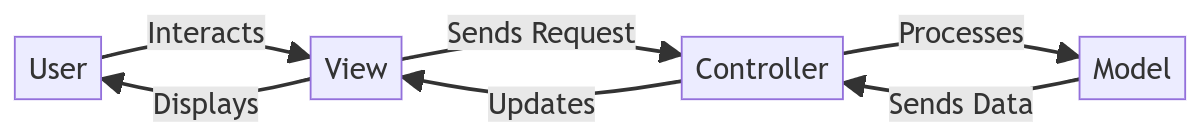
\includegraphics[width=\textwidth]{../figures/mvc-modern.png}
	\caption{Model View Controller Architecture}
	\label{fig:mvc_architecture}
\end{figure}

Pengguna berinteraksi dengan aplikasi melalui antarmuka pengguna yang dikenal sebagai View. View mencakup elemen-elemen seperti tombol, formulir, tabel, dan komponen visual lainnya yang memungkinkan pengguna memberikan input dan menerima output dari aplikasi. Sebagai contoh, dalam JavaFX, pengguna dapat mengklik tombol "Submit" pada sebuah formulir untuk memulai suatu aksi.

Ketika pengguna melakukan suatu aksi pada View, seperti mengklik tombol atau memasukkan teks, View akan mengirimkan permintaan tersebut ke Controller. View tidak menangani logika pemrosesan sendiri, melainkan menyerahkan tugas tersebut kepada Controller. Dalam JavaFX, View dapat memicu metode di Controller melalui event handler seperti \texttt{onAction} pada sebuah tombol.

Controller menerima permintaan dari View dan kemudian memprosesnya dengan berinteraksi dengan Model. Model adalah komponen yang bertanggung jawab atas logika bisnis dan operasi data, seperti mengakses database, melakukan perhitungan, atau memanipulasi data aplikasi. Sebagai contoh, Controller dapat memanggil metode di Model untuk mendapatkan daftar produk dari database.

Setelah Model selesai memproses permintaan, Model akan mengirimkan data kembali ke Controller. Data ini bisa berupa hasil query dari database, hasil perhitungan, atau data yang telah diproses sesuai logika bisnis. Dalam JavaFX, Model mungkin mengembalikan daftar objek yang kemudian dapat digunakan oleh Controller untuk memperbarui tampilan aplikasi.

Controller kemudian mengambil data dari Model dan memperbarui View sesuai dengan data tersebut. Pembaruan ini mungkin melibatkan pengisian tabel dengan data baru, memperbarui teks di label, atau menampilkan notifikasi kepada pengguna. Sebagai contoh, Controller di JavaFX dapat memperbarui elemen \texttt{TableView} dengan data terbaru yang diterima dari Model.

Terakhir, View akan menampilkan data yang telah diperbarui kepada pengguna. Pengguna kemudian dapat melihat hasil dari aksi yang mereka lakukan sebelumnya, seperti melihat tabel produk yang sudah terisi dengan data terbaru. Proses ini menciptakan siklus interaksi antara pengguna dan aplikasi, di mana setiap aksi pengguna dapat memicu pembaruan View melalui Controller dan Model.


\section{Prasyarat Java dan MySQL}
Sebelum memulai pengembangan aplikasi JavaFX, pastikan bahwa perangkat lunak berikut telah terinstal:

\begin{itemize}
	\item Java Development Kit (JDK) minimal versi 11 atau lebih baru.
	\item MySQL sebagai basis data untuk penyimpanan data aplikasi.
	\item Driver JDBC MySQL agar Java dapat berkomunikasi dengan database.
	\item Gradle sebagai build tool untuk mengelola dependensi dan otomasi proses pembangunan proyek.
\end{itemize}

\section{Mengunduh dan Menginstal Gradle serta Konfigurasi Proyek Java dengan Gradle}

Gradle adalah alat otomatisasi pembangunan proyek yang banyak digunakan dalam pengembangan perangkat lunak modern. Untuk menginstalnya, unduh versi terbaru dari situs resmi Gradle dan pastikan variabel lingkungan telah dikonfigurasi dengan benar agar dapat diakses melalui terminal. Untuk menginstal Gradle di sistem berbasis Linux, ikuti pentunjuk pada tautan berikut \url{https://gradle.org/install/}.


Langkah-langkah untuk menginisialisasi proyek Java dengan Gradle:

\begin{enumerate}
\item Pastikan Gradle telah terinstal dengan menjalankan perintah berikut:
\begin{lstlisting}[language=bash]
gradle -v
\end{lstlisting}

\item Buat direktori proyek baru dan masuk ke dalamnya:
\begin{lstlisting}[language=bash]
mkdir my-java-project
cd my-java-project
\end{lstlisting}

\item Jalankan perintah berikut untuk menginisialisasi proyek Java dengan Gradle:
\begin{lstlisting}[language=bash]
gradle init --type java-application
\end{lstlisting}
\end{enumerate}

Dengan perintah di atas, Gradle akan langsung menginisialisasi proyek Java sebagai aplikasi, tanpa perlu memilih opsi secara manual. Proyek Java dengan Gradle telah berhasil dikonfigurasi dan siap digunakan untuk pengembangan aplikasi berbasis Java.

\section{Struktur Direktori Proyek}
Setelah Gradle dikonfigurasi, target \texttt{folder} dan \texttt{files} yang akan dibuat dalam proyek ini adalah sebagai berikut.

\begin{lstlisting}[language=bash]
	my-javafx-project/
	|-- app/
	|   |-- build.gradle
	|   |-- src/
	|   |   |-- main/
	|   |   |   |-- java/
	|   |   |   |   |-- org/example/controllers/
	|   |   |   |   |   |-- ItemController.java
	|   |   |   |   |   |-- MainController.java
	|   |   |   |   |   |-- SalesOrderController.java
	|   |   |   |   |   |-- SelectFormController.java
	|   |   |   |   |-- org/example/helpers/
	|   |   |   |   |   |-- IForm.java
	|   |   |   |   |-- org/example/models/
	|   |   |   |   |   |-- Item.java
	|   |   |   |   |   |-- Order.java
	|   |   |   |   |   |-- OrderDetail.java
	|   |   |   |   |   |-- OrderDetailPK.java
	|   |   |   |-- resources/
	|   |   |   |   |-- hibernate.cfg.xml
	|   |   |   |   |-- Item.fxml
	|   |   |   |   |-- Main.fxml
	|   |   |   |   |-- SalesOrder.fxml
	|   |   |   |   |-- SelectForm.fxml
	|   |   |   |   |-- test.rptdesign
	|-- settings.gradle
	|-- gradle.properties
	|-- gradlew
	|-- gradlew.bat
\end{lstlisting}


Struktur proyek JavaFX ini terdiri dari beberapa direktori dan file utama yang dikelompokkan berdasarkan fungsinya. Berikut adalah target direktori dan file yang digunakan dalam proyek ini:

\begin{enumerate}
	\item \textbf{Root Direktori}:
	\begin{itemize}
		\item \texttt{settings.gradle} - File konfigurasi Gradle yang mengatur pengelolaan proyek multi-modul.
		\item \texttt{gradle.properties} - File properti Gradle yang menyimpan konfigurasi global proyek.
		\item \texttt{gradlew} dan \texttt{gradlew.bat} - Skrip untuk menjalankan Gradle Wrapper di sistem Unix dan Windows.
	\end{itemize}
	
	\item \textbf{Direktori Aplikasi (app/)}:
	\begin{itemize}
		\item \texttt{build.gradle} - File konfigurasi Gradle yang mengelola dependensi dan pengaturan proyek aplikasi.
		\item \texttt{src/} - Direktori utama yang berisi kode sumber proyek.
	\end{itemize}
	
	\item \textbf{Direktori Kode Sumber (src/main/)}:
	\begin{itemize}
		\item \texttt{java/org/example/controllers/} - Berisi kelas \textbf{Controller} yang menangani logika aplikasi, seperti \texttt{ItemController.java}, \texttt{MainController.java}, dan lainnya.
		\item \texttt{java/org/example/helpers/} - Berisi kelas bantuan yang mendukung operasi aplikasi, seperti \texttt{IForm.java}.
		\item \texttt{java/org/example/models/} - Berisi \textbf{Model} data yang merepresentasikan entitas bisnis, seperti \texttt{Item.java}, \texttt{Order.java}, dan \texttt{OrderDetail.java}.
	\end{itemize}
	
	\item \textbf{Direktori Resource (src/main/resources/)}:
	\begin{itemize}
		\item \texttt{hibernate.cfg.xml} - Konfigurasi Hibernate untuk menghubungkan aplikasi dengan database.
		\item Berkas \textbf{View} JavaFX dalam format \texttt{FXML}, seperti \texttt{Item.fxml}, \texttt{Main.fxml}, \texttt{SalesOrder.fxml}, dan \texttt{SelectForm.fxml}.
		\item \texttt{test.rptdesign} - Template laporan yang digunakan dalam aplikasi.
	\end{itemize}
\end{enumerate}


\section{Konfigurasi Gradle}

File \texttt{build.gradle} dalam proyek ini mengatur konfigurasi build menggunakan Gradle. Berikut adalah kode lengkap yang digunakan dalam file tersebut:

\begin{lstlisting}[style=JavaStyle]
	plugins {
		id 'application'
		id 'org.openjfx.javafxplugin' version '0.1.0'
	}
	
	repositories {
		mavenCentral()
	}
	
	dependencies {
		implementation 'mysql:mysql-connector-java:8.0.33'
		implementation 'org.hibernate:hibernate-core:6.2.12.Final'
		implementation 'jakarta.persistence:jakarta.persistence-api:3.1.0'
		implementation "org.openjfx:javafx-controls:20.0.1"
		implementation "org.openjfx:javafx-fxml:20.0.1"
		implementation 'com.innoventsolutions.birt.runtime:org.eclipse.birt.runtime_4.8.0-20180626:4.8.0'
		
		testImplementation libs.junit.jupiter
		testRuntimeOnly 'org.junit.platform:junit-platform-launcher'
		implementation libs.guava
	}
	
	java {
		toolchain {
			languageVersion = JavaLanguageVersion.of(21)
		}
	}
	
	application {
		mainClass = 'org.example.Main'
	}
	
	tasks.named('test') {
		useJUnitPlatform()
	}
	
	javafx {
		version = "21.0.1"
		modules = [ 'javafx.controls', 'javafx.fxml' ]
	}
\end{lstlisting}

Bagian \texttt{plugins} mendefinisikan plugin yang digunakan dalam proyek. Plugin \texttt{application} digunakan untuk aplikasi Java biasa, sedangkan \texttt{org.openjfx.javafxplugin} digunakan untuk mendukung JavaFX.

Bagian \texttt{repositories} menentukan lokasi tempat dependensi akan diunduh. Dalam konfigurasi ini, proyek menggunakan \texttt{mavenCentral()} sebagai repositori utama.

Bagian \texttt{dependencies} mendefinisikan pustaka eksternal yang digunakan dalam proyek. MySQL Connector digunakan untuk koneksi ke database MySQL. Hibernate Core digunakan untuk Object-Relational Mapping (ORM) dan manajemen database. Jakarta Persistence API merupakan API standar untuk ORM berbasis Java. JavaFX Controls dan JavaFX FXML menyediakan komponen antarmuka pengguna untuk JavaFX. BIRT Runtime digunakan untuk rendering laporan dalam aplikasi. JUnit dan Guava digunakan untuk pengujian unit dan utilitas tambahan dalam Java.

Bagian \texttt{java.toolchain} memastikan bahwa proyek menggunakan Java 21 sebagai versi bahasa pemrograman yang dikompilasi. Bagian \texttt{application} mendefinisikan kelas utama yang akan dijalankan dalam aplikasi, dalam hal ini \texttt{org.example.Main}. Bagian \texttt{tasks.named('test')} mengonfigurasi Gradle untuk menggunakan JUnit Platform sebagai framework pengujian. Bagian \texttt{javafx} menentukan versi JavaFX yang digunakan serta modul yang diperlukan dalam aplikasi.

\section{Konfigurasi Hibernate}

File \texttt{hibernate.cfg.xml} digunakan untuk mengonfigurasi Hibernate sebagai ORM (Object-Relational Mapping) yang menghubungkan aplikasi Java dengan database MySQL. Berikut adalah kode konfigurasi yang digunakan:

\begin{lstlisting}[style=XmlStyle]
	<?xml version="1.0" encoding="utf-8"?>
	<!DOCTYPE hibernate-configuration PUBLIC 
	"-//Hibernate/Hibernate Configuration DTD 3.0//EN"
	"http://www.hibernate.org/dtd/hibernate-configuration-3.0.dtd">
	<hibernate-configuration>
	<session-factory>
	<!-- Database Configuration -->
	<property name="hibernate.connection.driver_class">com.mysql.cj.jdbc.Driver</property>
	<property name="hibernate.connection.url">jdbc:mysql://localhost:3306/pradita?useSSL=false&amp;serverTimezone=UTC</property>
	<property name="hibernate.connection.username">alfa</property>
	<property name="hibernate.connection.password">1234</property>
	
	<!-- Hibernate Settings -->
	<property name="hibernate.dialect">org.hibernate.dialect.MySQLDialect</property>
	<property name="hibernate.show_sql">true</property>
	<property name="hibernate.format_sql">true</property>
	<property name="hibernate.hbm2ddl.auto">update</property>
	
	<!-- Entity Mappings -->
	<mapping class="org.example.models.Order"/>
	<mapping class="org.example.models.OrderDetail"/>
	<mapping class="org.example.models.Item"/>
	</session-factory>
	</hibernate-configuration>
\end{lstlisting}

Konfigurasi ini terdiri dari beberapa bagian utama yang mengatur koneksi database, konfigurasi Hibernate, dan pemetaan entitas.

Bagian pertama adalah pengaturan koneksi ke database MySQL, termasuk driver yang digunakan, URL koneksi, username, dan password. Database yang digunakan dalam konfigurasi ini adalah \texttt{pradita} yang berada di \texttt{localhost} dengan timezone UTC dan tanpa SSL. Parameter \texttt{hibernate.connection.driver\_class} menentukan driver JDBC untuk MySQL. \texttt{hibernate.connection.url} berisi alamat database, sedangkan \texttt{hibernate.connection.username} dan \texttt{hibernate.connection.password} digunakan untuk autentikasi koneksi.

Bagian berikutnya adalah pengaturan Hibernate yang mencakup beberapa properti utama. \texttt{hibernate.dialect} menentukan dialect SQL yang digunakan, dalam hal ini \texttt{MySQLDialect}, agar Hibernate dapat menghasilkan query yang sesuai dengan MySQL. \texttt{hibernate.show\_sql} diatur ke \texttt{true} agar semua query SQL yang dieksekusi dapat dilihat di log, sedangkan \texttt{hibernate.format\_sql} digunakan untuk menampilkan query dalam format yang lebih rapi. Opsi \texttt{hibernate.hbm2ddl.auto} diset ke \texttt{update}, yang memungkinkan Hibernate secara otomatis menyesuaikan struktur tabel database dengan entitas Java.

Bagian terakhir adalah pemetaan entitas yang menentukan kelas-kelas model dalam paket \texttt{org.example.models} yang akan dikelola oleh Hibernate. Konfigurasi ini mencakup tiga kelas utama, yaitu \texttt{Order}, \texttt{OrderDetail}, dan \texttt{Item}. Dengan pengaturan ini, Hibernate dapat menghubungkan kelas-kelas model dengan tabel dalam database secara otomatis dan melakukan operasi CRUD tanpa perlu menulis query SQL manual.

\section{Models}
Dalam arsitektur perangkat lunak berbasis Model-View-Controller (MVC), \textbf{Model} berperan sebagai representasi data dan logika bisnis yang berinteraksi langsung dengan database. Model bertanggung jawab untuk menyimpan, mengelola, dan memanipulasi data yang digunakan dalam aplikasi. Dengan menggunakan Hibernate sebagai ORM (Object-Relational Mapping), setiap entitas dalam model dipetakan ke dalam tabel database, memungkinkan operasi \textbf{CRUD (Create, Read, Update, Delete)} dilakukan secara efisien tanpa perlu menulis query SQL secara manual. Setiap model dalam aplikasi didefinisikan sebagai kelas Java dengan anotasi \texttt{jakarta.persistence} untuk mendeklarasikan hubungan antara atribut dalam kode dengan kolom dalam tabel database. Bagian ini akan membahas berbagai entitas dalam aplikasi, termasuk \texttt{Item}, \texttt{Order}, dan \texttt{OrderDetail}, serta bagaimana masing-masing kelas diimplementasikan dalam Hibernate.

\subsection{Item.java}

File \texttt{Item.java} merupakan kelas entitas yang dipetakan ke tabel \texttt{item} dalam database menggunakan Hibernate. Berikut adalah kode sumbernya:

\begin{lstlisting}[style=JavaStyle]
	package org.example.models;
	
	import jakarta.persistence.Column;
	import jakarta.persistence.Entity;
	import jakarta.persistence.Id;
	import jakarta.persistence.Table;
	
	@Entity
	@Table(name = "item")
	public class Item {
		@Id
		@Column(name = "code", length = 5, nullable = false)
		private String code;
		
		@Column(name = "name", length = 50)
		private String name;
		
		@Column(name = "price", nullable = false)
		private Double price;
		
		@Column(name = "quantity", nullable = false)
		private Double quantity;
		
		// Getters and setters
		public String getCode() { return code; }
		public void setCode(String code) { this.code = code; }
		
		public String getName() { return name; }
		public void setName(String name) { this.name = name; }
		
		public Double getPrice() { return price; }
		public void setPrice(Double price) { this.price = price; }
		
		public Double getQuantity() { return quantity; }
		public void setQuantity(Double quantity) { this.quantity = quantity; }
	}
\end{lstlisting}

Kelas \texttt{Item} menggunakan beberapa anotasi dari \texttt{jakarta.persistence} yang memungkinkan Hibernate untuk memetakan objek Java ke tabel database. \textbf{Setiap anotasi memiliki fungsi spesifik} dalam proses ORM (Object-Relational Mapping) yang dilakukan oleh Hibernate.

\begin{enumerate}
	\item \textbf{Anotasi \texttt{@Entity}}. 
	Anotasi \texttt{@Entity} menandakan bahwa kelas ini merupakan entitas yang akan dipetakan ke dalam tabel database. Hibernate akan mengelola objek dari kelas ini dan menyimpannya dalam database.
	
	\item \textbf{Anotasi \texttt{@Table(name = \"item\")}}. 
	Anotasi \texttt{@Table(name = "item")} mengaitkan kelas \texttt{Item} dengan tabel \texttt{item} dalam database. Jika anotasi ini tidak diberikan, secara default Hibernate akan menggunakan nama kelas sebagai nama tabel.
	
	\item \textbf{Anotasi \texttt{@Id}}. 
	Atribut \texttt{code} digunakan sebagai primary key dari tabel \texttt{item}. Anotasi \texttt{@Id} menandakan bahwa atribut ini adalah kolom unik yang digunakan oleh Hibernate untuk mengidentifikasi setiap entitas dalam database.
	
	\item \textbf{Anotasi \texttt{@Column}}.
	Anotasi \texttt{@Column} digunakan untuk mendefinisikan properti yang akan dipetakan ke dalam kolom tabel database:
	\begin{enumerate}
		\item \texttt{@Column(name = "code", length = 5, nullable = false)} - Kolom \texttt{code} memiliki panjang maksimum 5 karakter dan tidak boleh kosong (\texttt{nullable = false}). Properti ini berfungsi sebagai primary key.
		\item \texttt{@Column(name = "name", length = 50)} - Kolom \texttt{name} memiliki panjang maksimum 50 karakter. Tidak ada batasan \texttt{nullable}, sehingga dapat diisi atau dibiarkan kosong.
		\item \texttt{@Column(name = "price", nullable = false)} - Kolom \texttt{price} menggunakan tipe data \texttt{Double} dan wajib diisi (\texttt{nullable = false}).
		\item \texttt{@Column(name = "quantity", nullable = false)} - Kolom \texttt{quantity} juga menggunakan tipe data \texttt{Double} dan wajib diisi (\texttt{nullable = false}).
	\end{enumerate}
	
	\item \textbf{Penggunaan Getter dan Setter}.
	Setiap atribut memiliki metode getter dan setter. Hibernate membutuhkan metode ini untuk membaca dan memperbarui nilai dari setiap atribut saat melakukan operasi database.

\end{enumerate}

Dengan konfigurasi ini, Hibernate akan melakukan pemetaan tabel \texttt{item} sebagai berikut:
\begin{enumerate}
	\item Setiap objek \texttt{Item} akan diperlakukan sebagai satu baris data dalam tabel \texttt{item}.
	\item Jika sebuah objek \texttt{Item} disimpan menggunakan Hibernate, maka Hibernate akan mengeksekusi query \texttt{INSERT} ke dalam database.
	\item Jika sebuah objek \texttt{Item} diubah, Hibernate akan secara otomatis menjalankan query \texttt{UPDATE} untuk menyimpan perubahan tersebut.
	\item Jika sebuah objek \texttt{Item} dihapus, Hibernate akan menjalankan query \texttt{DELETE}.
\end{enumerate}

Sebagai contoh, ketika kita menyimpan objek baru menggunakan Hibernate:

\begin{lstlisting}[style=JavaStyle]
	Session session = HibernateUtil.getSessionFactory().openSession();
	Transaction transaction = session.beginTransaction();
	
	Item item = new Item();
	item.setCode("A123");
	item.setName("Laptop");
	item.setPrice(15000000.0);
	item.setQuantity(10.0);
	
	session.save(item);
	transaction.commit();
	session.close();
\end{lstlisting}

Kode di atas akan menyebabkan Hibernate mengeksekusi query berikut dalam database:

\begin{lstlisting}[style=sql]
	INSERT INTO item (code, name, price, quantity) 
	VALUES ('A123', 'Laptop', 15000000.0, 10.0);
\end{lstlisting}

Jika kita ingin mengambil data berdasarkan kode barang:

\begin{lstlisting}[style=JavaStyle]
	Session session = HibernateUtil.getSessionFactory().openSession();
	Item item = session.get(Item.class, "A123");
	System.out.println("Nama Barang: " + item.getName());
	session.close();
\end{lstlisting}

Hibernate akan menerjemahkannya ke dalam query SQL berikut:

\begin{lstlisting}[style=sql]
	SELECT * FROM item WHERE code = 'A123';
\end{lstlisting}

Dengan pemetaan ini, Hibernate dapat menangani interaksi dengan database secara otomatis tanpa perlu menulis query SQL secara manual. Hal ini membuat pengelolaan database lebih efisien dan mengurangi ketergantungan pada query SQL yang eksplisit.


\subsection{Order.java}

File \texttt{Order.java} merupakan kelas entitas yang dipetakan ke tabel \texttt{order} dalam database menggunakan Hibernate. Kelas ini berfungsi sebagai model yang merepresentasikan pesanan dalam aplikasi. Berikut adalah kode sumbernya:

\begin{lstlisting}[style=JavaStyle]
	package org.example.models;
	
	import java.time.LocalDateTime;
	import java.util.List;
	
	import jakarta.persistence.CascadeType;
	import jakarta.persistence.Column;
	import jakarta.persistence.Entity;
	import jakarta.persistence.Id;
	import jakarta.persistence.OneToMany;
	import jakarta.persistence.Table;
	
	@Entity
	@Table(name = "order")
	public class Order {
		@Id
		@Column(name = "code", length = 5, nullable = false)
		private String code;
		
		@Column(name = "note", columnDefinition = "TEXT")
		private String note;
		
		@Column(name = "date", columnDefinition = "DATETIME DEFAULT CURRENT_TIMESTAMP")
		private LocalDateTime date;
		
		@OneToMany(mappedBy = "order", cascade = CascadeType.ALL, orphanRemoval = true)
		private List<OrderDetail> orderDetails;
		
		// Getters and setters
		public String getCode() { return code; }
		public void setCode(String code) { this.code = code; }
		
		public String getNote() { return note; }
		public void setNote(String note) { this.note = note; }
		
		public LocalDateTime getDate() { return date; }
		public void setDate(LocalDateTime date) { this.date = date; }
		
		public List<OrderDetail> getOrderDetails() { return orderDetails; }
		public void setOrderDetails(List<OrderDetail> orderDetails) { this.orderDetails = orderDetails; }
	}
\end{lstlisting}

Kelas \texttt{Order} menggunakan beberapa anotasi dari \texttt{jakarta.persistence} yang memungkinkan Hibernate untuk memetakan objek Java ke tabel database.

\begin{enumerate}
	\item \textbf{Anotasi \texttt{@Entity}}. 
	Anotasi \texttt{@Entity} menandakan bahwa kelas ini merupakan entitas yang akan dipetakan ke dalam tabel database. Hibernate akan mengelola objek dari kelas ini dan menyimpannya dalam database.
	
	\item \textbf{Anotasi \texttt{@Table(name = "order")}}. 
	Anotasi \texttt{@Table(name = "order")} mengaitkan kelas \texttt{Order} dengan tabel \texttt{order} dalam database. Jika anotasi ini tidak diberikan, secara default Hibernate akan menggunakan nama kelas sebagai nama tabel.
	
	\item \textbf{Anotasi \texttt{@Id}}. 
	Atribut \texttt{code} digunakan sebagai primary key dari tabel \texttt{order}. Anotasi \texttt{@Id} menandakan bahwa atribut ini adalah kolom unik yang digunakan oleh Hibernate untuk mengidentifikasi setiap entitas dalam database.
	
	\item \textbf{Anotasi \texttt{@Column}}.
	Anotasi \texttt{@Column} digunakan untuk mendefinisikan properti yang akan dipetakan ke dalam kolom tabel database:
	\begin{enumerate}
		\item \texttt{@Column(name = "code", length = 5, nullable = false)} - Kolom \texttt{code} memiliki panjang maksimum 5 karakter dan tidak boleh kosong (\texttt{nullable = false}). Properti ini berfungsi sebagai primary key.
		\item \texttt{@Column(name = "note", columnDefinition = "TEXT")} - Kolom \texttt{note} digunakan untuk menyimpan catatan pesanan dalam format teks panjang.
		\item \texttt{@Column(name = "date", columnDefinition = "DATETIME DEFAULT CURRENT\_TIMESTAMP")} - Kolom \texttt{date} menyimpan waktu pembuatan pesanan dengan nilai default \texttt{CURRENT\_TIMESTAMP}.
	\end{enumerate}
	
	\item \textbf{Anotasi \texttt{@OneToMany}}.
	Atribut \texttt{orderDetails} direpresentasikan sebagai daftar (\texttt{List}) yang berisi \texttt{OrderDetail}. 
	\begin{enumerate}
		\item \texttt{@OneToMany(mappedBy = "order", cascade = CascadeType.ALL, orphanRemoval = true)} \\
		Anotasi ini menunjukkan bahwa hubungan antara \texttt{Order} dan \texttt{OrderDetail} adalah **one-to-many**.
		\begin{itemize}
			\item \texttt{mappedBy = "order"} - Menunjukkan bahwa hubungan ini dikendalikan oleh atribut \texttt{order} dalam kelas \texttt{OrderDetail}.
			\item \texttt{cascade = CascadeType.ALL} - Jika entitas \texttt{Order} dibuat, diperbarui, atau dihapus, maka semua \texttt{OrderDetail} yang terkait akan ikut diperbarui atau dihapus.
			\item \texttt{orphanRemoval = true} - Jika sebuah \texttt{OrderDetail} tidak lagi terkait dengan entitas \texttt{Order}, maka entitas tersebut akan dihapus dari database.
		\end{itemize}
	\end{enumerate}
	
	\item \textbf{Penggunaan Getter dan Setter}.
	Setiap atribut memiliki metode getter dan setter. Hibernate membutuhkan metode ini untuk membaca dan memperbarui nilai dari setiap atribut saat melakukan operasi database.
	
\end{enumerate}

Dengan konfigurasi ini, Hibernate akan melakukan pemetaan tabel \texttt{order} sebagai berikut:
\begin{enumerate}
	\item Setiap objek \texttt{Order} akan diperlakukan sebagai satu baris data dalam tabel \texttt{order}.
	\item Jika sebuah objek \texttt{Order} disimpan menggunakan Hibernate, maka Hibernate akan mengeksekusi query \texttt{INSERT} ke dalam database.
	\item Jika sebuah objek \texttt{Order} diubah, Hibernate akan secara otomatis menjalankan query \texttt{UPDATE} untuk menyimpan perubahan tersebut.
	\item Jika sebuah objek \texttt{Order} dihapus, Hibernate akan menjalankan query \texttt{DELETE}.
\end{enumerate}

Sebagai contoh, ketika kita menyimpan objek baru menggunakan Hibernate:

\begin{lstlisting}[style=JavaStyle]
	Session session = HibernateUtil.getSessionFactory().openSession();
	Transaction transaction = session.beginTransaction();
	
	Order order = new Order();
	order.setCode("O123");
	order.setNote("Pesanan pertama");
	order.setDate(LocalDateTime.now());
	
	session.save(order);
	transaction.commit();
	session.close();
\end{lstlisting}

Kode di atas akan menyebabkan Hibernate mengeksekusi query berikut dalam database:

\begin{lstlisting}[style=sql]
	INSERT INTO `order` (code, note, date) 
	VALUES ('O123', 'Pesanan pertama', CURRENT_TIMESTAMP);
\end{lstlisting}

Jika kita ingin mengambil data berdasarkan kode pesanan:

\begin{lstlisting}[style=JavaStyle]
	Session session = HibernateUtil.getSessionFactory().openSession();
	Order order = session.get(Order.class, "O123");
	System.out.println("Catatan Pesanan: " + order.getNote());
	session.close();
\end{lstlisting}

Hibernate akan menerjemahkannya ke dalam query SQL berikut:

\begin{lstlisting}[style=sql]
	SELECT * FROM `order` WHERE code = 'O123';
\end{lstlisting}

Dengan pemetaan ini, Hibernate dapat menangani interaksi dengan database secara otomatis tanpa perlu menulis query SQL secara manual. Konfigurasi ini memastikan bahwa hubungan antara pesanan dan detail pesanan dapat dikelola dengan baik oleh Hibernate.


\subsection{OrderDetail.java}

File \texttt{OrderDetail.java} merupakan kelas entitas yang dipetakan ke tabel \texttt{order\_detail} dalam database menggunakan Hibernate. Kelas ini menyimpan detail pesanan yang terkait dengan pesanan utama dalam aplikasi. Berikut adalah kode sumbernya:

\begin{lstlisting}[style=JavaStyle]
	package org.example.models;
	
	import jakarta.persistence.Column;
	import jakarta.persistence.EmbeddedId;
	import jakarta.persistence.Entity;
	import jakarta.persistence.JoinColumn;
	import jakarta.persistence.ManyToOne;
	import jakarta.persistence.MapsId;
	import jakarta.persistence.Table;
	
	@Entity
	@Table(name = "order_detail")
	public class OrderDetail {
		@EmbeddedId
		private OrderDetailPK id;
		
		@ManyToOne
		@MapsId("orderCode")
		@JoinColumn(name = "code", nullable = false)
		private Order order;
		
		@Column(name = "itemcode", length = 5, nullable = false)
		private String itemCode;
		
		@Column(name = "name", length = 50)
		private String name;
		
		@Column(name = "price", nullable = false)
		private Double price;
		
		@Column(name = "quantity", nullable = false)
		private Double quantity;
		
		public OrderDetail() {}
		
		public OrderDetail(OrderDetailPK id, Order order, String itemCode, String name, double price, double quantity) {
			this.id = id;
			this.order = order;
			this.itemCode = itemCode;
			this.name = name;
			this.price = price;
			this.quantity = quantity;
		}
		
		// Getters and setters
		public OrderDetailPK getId() { return id; }
		public void setId(OrderDetailPK id) { this.id = id; }
		
		public Order getOrder() { return order; }
		public void setOrder(Order order) { this.order = order; }
		
		public String getItemCode() { return itemCode; }
		public void setItemCode(String itemCode) { this.itemCode = itemCode; }
		
		public String getName() { return name; }
		public void setName(String name) { this.name = name; }
		
		public Double getPrice() { return price; }
		public void setPrice(Double price) { this.price = price; }
		
		public Double getQuantity() { return quantity; }
		public void setQuantity(Double quantity) { this.quantity = quantity; }
	}
\end{lstlisting}

Kelas \texttt{OrderDetail} menggunakan beberapa anotasi dari \texttt{jakarta.persistence} yang memungkinkan Hibernate untuk memetakan objek Java ke tabel database.

\begin{enumerate}
	\item \textbf{Anotasi \texttt{@Entity}}. 
	Anotasi \texttt{@Entity} menandakan bahwa kelas ini merupakan entitas yang akan dipetakan ke dalam tabel database. Hibernate akan mengelola objek dari kelas ini dan menyimpannya dalam database.
	
	\item \textbf{Anotasi \texttt{@Table(name = "order\_detail")}}. 
	Anotasi \texttt{@Table(name = "order\_detail")} mengaitkan kelas \texttt{OrderDetail} dengan tabel \texttt{order\_detail} dalam database.
	
	\item \textbf{Anotasi \texttt{@EmbeddedId}}. 
	Anotasi \texttt{@EmbeddedId} menunjukkan bahwa primary key dari entitas ini terdiri dari beberapa kolom yang dikelola dalam kelas \texttt{OrderDetailPK}.
	
	\item \textbf{Anotasi \texttt{@ManyToOne}}. 
	Anotasi \texttt{@ManyToOne} menunjukkan bahwa entitas ini memiliki relasi **many-to-one** dengan \texttt{Order}, di mana banyak \texttt{OrderDetail} dapat terkait dengan satu \texttt{Order}.
	
	\item \textbf{Anotasi \texttt{@MapsId}}. 
	Anotasi \texttt{@MapsId("orderCode")} menunjukkan bahwa nilai primary key dari \texttt{OrderDetail} akan menggunakan primary key dari \texttt{Order}.
	
	\item \textbf{Anotasi \texttt{@JoinColumn}}. 
	Anotasi \texttt{@JoinColumn(name = "code", nullable = false)} menentukan bahwa kolom \texttt{code} adalah foreign key yang menghubungkan entitas ini dengan tabel \texttt{order}.
	
	\item \textbf{Anotasi \texttt{@Column}}. 
	Anotasi \texttt{@Column} digunakan untuk mendefinisikan properti yang akan dipetakan ke dalam kolom tabel database:
	\begin{enumerate}
		\item \texttt{@Column(name = "itemcode", length = 5, nullable = false)} - Kolom \texttt{itemcode} menyimpan kode item dengan panjang maksimum 5 karakter dan tidak boleh kosong.
		\item \texttt{@Column(name = "name", length = 50)} - Kolom \texttt{name} menyimpan nama item dengan panjang maksimum 50 karakter.
		\item \texttt{@Column(name = "price", nullable = false)} - Kolom \texttt{price} menyimpan harga item dan wajib diisi.
		\item \texttt{@Column(name = "quantity", nullable = false)} - Kolom \texttt{quantity} menyimpan jumlah item dan wajib diisi.
	\end{enumerate}
	
	\item \textbf{Penggunaan Getter dan Setter}. 
	Setiap atribut memiliki metode getter dan setter. Hibernate membutuhkan metode ini untuk membaca dan memperbarui nilai dari setiap atribut saat melakukan operasi database.
\end{enumerate}

Dengan konfigurasi ini, Hibernate akan melakukan pemetaan tabel \texttt{order\_detail} sebagai berikut:
\begin{enumerate}
	\item Setiap objek \texttt{OrderDetail} akan diperlakukan sebagai satu baris data dalam tabel \texttt{order\_detail}.
	\item Jika sebuah objek \texttt{OrderDetail} disimpan menggunakan Hibernate, maka Hibernate akan mengeksekusi query \texttt{INSERT} ke dalam database.
	\item Jika sebuah objek \texttt{OrderDetail} diubah, Hibernate akan secara otomatis menjalankan query \texttt{UPDATE} untuk menyimpan perubahan tersebut.
	\item Jika sebuah objek \texttt{OrderDetail} dihapus, Hibernate akan menjalankan query \texttt{DELETE}.
\end{enumerate}

Sebagai contoh, ketika kita menyimpan objek baru menggunakan Hibernate:

\begin{lstlisting}[style=JavaStyle]
	Session session = HibernateUtil.getSessionFactory().openSession();
	Transaction transaction = session.beginTransaction();
	
	OrderDetailPK id = new OrderDetailPK("O123", "I567");
	Order order = session.get(Order.class, "O123");
	OrderDetail orderDetail = new OrderDetail(id, order, "I567", "Mouse", 50000.0, 2.0);
	
	session.save(orderDetail);
	transaction.commit();
	session.close();
\end{lstlisting}

Kode di atas akan menyebabkan Hibernate mengeksekusi query berikut dalam database:

\begin{lstlisting}[style=sql]
	INSERT INTO order_detail (code, itemcode, name, price, quantity) 
	VALUES ('O123', 'I567', 'Mouse', 50000.0, 2.0);
\end{lstlisting}

Dengan pemetaan ini, Hibernate dapat menangani interaksi dengan database secara otomatis tanpa perlu menulis query SQL secara manual. Konfigurasi ini memastikan bahwa hubungan antara detail pesanan dan pesanan utama dapat dikelola dengan baik oleh Hibernate.


\subsection{OrderDetailPK.java}

File \texttt{OrderDetailPK.java} merupakan kelas yang digunakan sebagai \textbf{primary key} komposit dalam entitas \texttt{OrderDetail}. Kelas ini berfungsi sebagai identifier unik yang terdiri dari beberapa kolom dalam tabel \texttt{order\_detail}. Berikut adalah kode sumbernya:

\begin{lstlisting}[style=JavaStyle]
	package org.example.models;
	
	import java.util.Objects;
	import jakarta.persistence.Column;
	import jakarta.persistence.Embeddable;
	
	@Embeddable
	public class OrderDetailPK implements java.io.Serializable {
		@Column(name = "code", length = 5, nullable = false)
		private String orderCode;
		
		@Column(name = "line", nullable = false)
		private Integer line;
		
		public OrderDetailPK() {}
		
		public OrderDetailPK(String newCode, int line) {
			this.orderCode = newCode;
			this.line = line;
		}
		
		// Getters, setters, equals, and hashCode
		public String getOrderCode() { return orderCode; }
		public void setOrderCode(String orderCode) { this.orderCode = orderCode; }
		
		public Integer getLine() { return line; }
		public void setLine(Integer line) { this.line = line; }
		
		@Override
		public boolean equals(Object o) {
			if (this == o) return true;
			if (o == null || getClass() != o.getClass()) return false;
			OrderDetailPK that = (OrderDetailPK) o;
			return Objects.equals(orderCode, that.orderCode) && Objects.equals(line, that.line);
		}
		
		@Override
		public int hashCode() {
			return Objects.hash(orderCode, line);
		}
	}
\end{lstlisting}

Kelas \texttt{OrderDetailPK} menggunakan beberapa anotasi dari \texttt{jakarta.persistence} yang memungkinkan Hibernate untuk menangani primary key komposit.

\begin{enumerate}
	\item \textbf{Anotasi \texttt{@Embeddable}}. 
	Anotasi \texttt{@Embeddable} menandakan bahwa kelas ini digunakan untuk menjadi bagian dari primary key dalam kelas entitas lain, dalam hal ini \texttt{OrderDetail}.
	
	\item \textbf{Anotasi \texttt{@Column}}. 
	Anotasi \texttt{@Column} digunakan untuk mendefinisikan properti yang akan dipetakan ke dalam kolom tabel database:
	\begin{enumerate}
		\item \texttt{@Column(name = "code", length = 5, nullable = false)} - Kolom \texttt{code} berisi kode pesanan sebagai bagian dari primary key.
		\item \texttt{@Column(name = "line", nullable = false)} - Kolom \texttt{line} berfungsi sebagai nomor baris dalam pesanan.
	\end{enumerate}
	
	\item \textbf{Implementasi Interface \texttt{Serializable}}. 
	Kelas ini mengimplementasikan \texttt{java.io.Serializable} agar dapat digunakan sebagai primary key dalam Hibernate. Hibernate membutuhkan primary key komposit untuk dapat diubah menjadi representasi byte-stream.
	
	\item \textbf{Implementasi Metode \texttt{equals} dan \texttt{hashCode}}. 
	\begin{enumerate}
		\item Metode \texttt{equals()} digunakan untuk membandingkan dua objek \texttt{OrderDetailPK} berdasarkan \texttt{orderCode} dan \texttt{line}.
		\item Metode \texttt{hashCode()} digunakan untuk menghasilkan nilai hash berdasarkan atribut \texttt{orderCode} dan \texttt{line}, yang berguna untuk memastikan integritas data dalam koleksi seperti \texttt{HashSet} atau \texttt{HashMap}.
	\end{enumerate}
\end{enumerate}

Dengan konfigurasi ini, Hibernate akan melakukan pemetaan tabel \texttt{order\_detail} sebagai berikut:
\begin{enumerate}
	\item Setiap objek \texttt{OrderDetailPK} akan digunakan sebagai kunci unik dalam tabel \texttt{order\_detail}.
	\item Jika sebuah objek \texttt{OrderDetail} disimpan menggunakan Hibernate, maka kunci yang digunakan adalah gabungan dari \texttt{code} dan \texttt{line}.
	\item Jika sebuah objek \texttt{OrderDetail} dihapus, Hibernate akan mencari data berdasarkan primary key komposit ini sebelum menjalankan query \texttt{DELETE}.
\end{enumerate}

Sebagai contoh, ketika kita menyimpan objek baru menggunakan Hibernate:

\begin{lstlisting}[style=JavaStyle]
	Session session = HibernateUtil.getSessionFactory().openSession();
	Transaction transaction = session.beginTransaction();
	
	OrderDetailPK id = new OrderDetailPK("O123", 1);
	Order order = session.get(Order.class, "O123");
	OrderDetail orderDetail = new OrderDetail(id, order, "I567", "Mouse", 50000.0, 2.0);
	
	session.save(orderDetail);
	transaction.commit();
	session.close();
\end{lstlisting}

Kode di atas akan menyebabkan Hibernate mengeksekusi query berikut dalam database:

\begin{lstlisting}[style=sql]
	INSERT INTO order_detail (code, line, itemcode, name, price, quantity) 
	VALUES ('O123', 1, 'I567', 'Mouse', 50000.0, 2.0);
\end{lstlisting}

Dengan pemetaan ini, Hibernate dapat menangani interaksi dengan database secara otomatis tanpa perlu menulis query SQL secara manual. Konfigurasi ini memastikan bahwa setiap detail pesanan memiliki primary key unik yang terdiri dari kode pesanan dan nomor baris.

\section{Controllers}


\subsection{MainController.java}

Dalam aplikasi berbasis JavaFX, kelas \texttt{MainController} bertindak sebagai pengendali utama yang mengelola interaksi pengguna dengan antarmuka grafis dan menangani berbagai operasi bisnis. Kelas ini bertanggung jawab untuk membuka berbagai formulir, menangani koneksi ke database MySQL, serta menangani pembuatan dan pencetakan laporan menggunakan BIRT (Business Intelligence and Reporting Tools). Dengan memanfaatkan mekanisme \textbf{FXML}, JavaFX dapat memisahkan tampilan dan logika bisnis, sehingga pengelolaan antarmuka menjadi lebih modular dan mudah dikembangkan.

Berikut adalah kode sumber dari kelas \texttt{MainController}:

\begin{lstlisting}[style=JavaStyle]
	package org.example.controllers;
	
	import java.awt.Desktop;
	import java.io.File;
	import java.io.IOException;
	import java.sql.Connection;
	import java.sql.DriverManager;
	
	import org.eclipse.birt.core.framework.Platform;
	import org.eclipse.birt.report.engine.api.EngineConfig;
	import org.eclipse.birt.report.engine.api.IReportEngine;
	import org.eclipse.birt.report.engine.api.IReportEngineFactory;
	import org.eclipse.birt.report.engine.api.IReportRunnable;
	import org.eclipse.birt.report.engine.api.IRunAndRenderTask;
	import org.eclipse.birt.report.engine.api.PDFRenderOption;
	import org.example.helpers.IForm;
	
	import javafx.fxml.FXML;
	import javafx.fxml.FXMLLoader;
	import javafx.scene.Parent;
	import javafx.scene.control.Alert;
	import javafx.scene.control.MenuItem;
	import javafx.scene.layout.BorderPane;
	
	public class MainController {
		
		@FXML
		private MenuItem menuItemPrint;
		@FXML
		private MenuItem menuItemClose;
		@FXML
		private MenuItem menuItemOpenItem;
		@FXML
		private MenuItem menuItemAbout;
		@FXML
		private MenuItem menuItemOpenSalesOrder;
		@FXML
		private BorderPane centerPane;
		public static Connection CONNECTION;
		
		private IForm currentForm;
		
		public void initialize() {
			System.out.println("Main Controller Initialized");
		}
		
		@FXML
		private void openItem() {
			try {
				FXMLLoader loader = new FXMLLoader(getClass().getResource("/Item.fxml"));
				Parent itemFormRoot = loader.load();
				centerPane.setCenter(itemFormRoot);
				currentForm = loader.getController();
			} catch (IOException e) {
				e.printStackTrace();
				showAlert("Error", "Could not open Item Form.");
			}
		}
		
		@FXML
		private void openSalesOrder() {
			try {
				FXMLLoader loader = new FXMLLoader(getClass().getResource("/SalesOrder.fxml"));
				Parent salesOrderRoot = loader.load();
				centerPane.setCenter(salesOrderRoot);
				currentForm = loader.getController();
			} catch (IOException e) {
				e.printStackTrace();
				showAlert("Error", "Could not open Sales Order Form.");
			}
		}
		
		@FXML
		private void showAbout() {
			Alert alert = new Alert(Alert.AlertType.INFORMATION);
			alert.setTitle("About");
			alert.setHeaderText("Order Form Application");
			alert.setContentText("Developed with JavaFX and BIRT for report generation.");
			alert.showAndWait();
		}
		
		@FXML
		private void printReport() {
			new Thread(() -> {
				try {
					EngineConfig config = new EngineConfig();
					Platform.startup(config);
					IReportEngineFactory factory = (IReportEngineFactory) Platform
					.createFactoryObject(IReportEngineFactory.EXTENSION_REPORT_ENGINE_FACTORY);
					IReportEngine engine = factory.createReportEngine(config);
					
					IReportRunnable design = engine.openReportDesign("/data2/projects/pemrograman-berorientasi-objek/code/pertemuan_05/javafx/app/build/resources/main/test.rptdesign");
					IRunAndRenderTask task = engine.createRunAndRenderTask(design);
					task.setParameterValue("order_code", currentForm.getDocumentCode());
					PDFRenderOption options = new PDFRenderOption();
					options.setOutputFileName("document.pdf");
					options.setOutputFormat("pdf");
					
					task.setRenderOption(options);
					task.run();
					task.close();
					engine.destroy();
					
					if (Desktop.isDesktopSupported()) {
						File myFile = new File("document.pdf");
						Desktop.getDesktop().open(myFile);
					}
					
				} catch (Exception e) {
					e.printStackTrace();
				} finally {
					Platform.shutdown();
				}
			}).start();
		}
		
		private void showAlert(String title, String message) {
			Alert alert = new Alert(Alert.AlertType.ERROR);
			alert.setTitle(title);
			alert.setHeaderText(null);
			alert.setContentText(message);
			alert.showAndWait();
		}
	}
\end{lstlisting}

Kelas \texttt{MainController} memiliki beberapa fungsi utama:

\begin{enumerate}
	
	\item \textbf{Membuka Formulir Item dan Sales Order}.  
	Aplikasi ini memungkinkan pengguna untuk membuka formulir yang berbeda dengan menggunakan metode \texttt{openItem()} dan \texttt{openSalesOrder()}. Kedua metode ini menggunakan \texttt{FXMLLoader} untuk memuat file \texttt{.fxml} yang berisi tampilan dan menampilkannya dalam \texttt{centerPane}. Referensi controller dari tampilan yang dibuka disimpan dalam variabel \texttt{currentForm}.
	
	\item \textbf{Menampilkan Dialog Informasi}.  
	Metode \texttt{showAbout()} menampilkan informasi tentang aplikasi menggunakan objek \texttt{Alert} dari JavaFX. Dialog ini menampilkan nama aplikasi dan informasi teknologi yang digunakan.
	
	\item \textbf{Pencetakan Laporan dengan BIRT}.  
	Metode \texttt{printReport()} digunakan untuk menghasilkan laporan dalam format PDF. Laporan dibuka menggunakan BIRT dengan \texttt{IReportEngine}, kemudian parameter laporan ditetapkan menggunakan \texttt{setParameterValue()}. Laporan dijalankan dan diekspor dalam format PDF dengan \texttt{PDFRenderOption}. Setelah selesai, jika sistem mendukung fitur desktop, file PDF akan dibuka secara otomatis.
	
	\item \textbf{Penanganan Kesalahan}.  
	Jika terjadi kesalahan dalam proses pemuatan tampilan atau pembuatan laporan, metode \texttt{showAlert()} digunakan untuk menampilkan pesan kesalahan kepada pengguna. Dialog kesalahan dibuat menggunakan objek \texttt{Alert} dari JavaFX.
\end{enumerate}

Dengan konfigurasi ini, \texttt{MainController} bertindak sebagai penghubung antara antarmuka pengguna dan logika bisnis dalam aplikasi. Kombinasi JavaFX dan BIRT memungkinkan aplikasi untuk menangani data dan menghasilkan laporan secara efektif. 

\subsection{ItemController.java}

Kelas \texttt{ItemController} berfungsi sebagai pengendali utama untuk tampilan dan manajemen data item dalam aplikasi berbasis JavaFX. Kelas ini bertanggung jawab untuk menampilkan daftar item dalam tabel, menangani perubahan data secara langsung melalui tabel, serta menyimpan perubahan ke dalam database menggunakan Hibernate. Integrasi antara JavaFX dan Hibernate memungkinkan data item dikelola dengan lebih efisien dan konsisten dalam aplikasi.

Berikut adalah kode sumber dari kelas \texttt{ItemController}:

\begin{lstlisting}[style=JavaStyle]
	package org.example.controllers;
	
	import java.util.List;
	
	import org.example.Main;
	import org.example.helpers.IForm;
	import org.hibernate.Session;
	import org.hibernate.Transaction;
	
	import javafx.beans.property.SimpleDoubleProperty;
	import javafx.beans.property.SimpleStringProperty;
	import javafx.collections.FXCollections;
	import javafx.collections.ObservableList;
	import javafx.fxml.FXML;
	import javafx.scene.control.TableColumn;
	import javafx.scene.control.TableView;
	import javafx.scene.control.cell.TextFieldTableCell;
	import javafx.util.converter.DoubleStringConverter;
	
	public class ItemController implements IForm {
		
		@FXML
		private TableView<Item> table;
		@FXML
		private TableColumn<Item, String> colCode;
		@FXML
		private TableColumn<Item, String> colName;
		@FXML
		private TableColumn<Item, Double> colPrice;
		@FXML
		private TableColumn<Item, Double> colQuantity;
		
		private ObservableList<Item> items = FXCollections.observableArrayList();
		
		public void initialize() {
			colCode.setCellValueFactory(cellData -> cellData.getValue().codeProperty());
			colName.setCellValueFactory(cellData -> cellData.getValue().nameProperty());
			colPrice.setCellValueFactory(cellData -> cellData.getValue().priceProperty().asObject());
			colQuantity.setCellValueFactory(cellData -> cellData.getValue().quantityProperty().asObject());
			
			table.setItems(items);
			table.setEditable(true);
			
			colCode.setCellFactory(TextFieldTableCell.forTableColumn());
			colName.setCellFactory(TextFieldTableCell.forTableColumn());
			colPrice.setCellFactory(TextFieldTableCell.forTableColumn(new DoubleStringConverter()));
			colQuantity.setCellFactory(TextFieldTableCell.forTableColumn(new DoubleStringConverter()));
			
			colCode.setOnEditCommit(event -> {
				Item item = event.getRowValue();
				item.setCode(event.getNewValue());
				handleTableEdit(item, "code");
			});
			
			colName.setOnEditCommit(event -> {
				Item item = event.getRowValue();
				item.setName(event.getNewValue());
				handleTableEdit(item, "name");
			});
			
			colPrice.setOnEditCommit(event -> {
				Item item = event.getRowValue();
				item.setPrice(event.getNewValue());
				handleTableEdit(item, "price");
			});
			
			colQuantity.setOnEditCommit(event -> {
				Item item = event.getRowValue();
				item.setQuantity(event.getNewValue());
				handleTableEdit(item, "quantity");
			});
			
			loadItems();
			items.add(new Item("", "", 0.0, 0.0));
		}
		
		private void loadItems() {
			try (Session session = Main.getSessionFactory().openSession()) {
				List<org.example.models.Item> itemList = session.createQuery("FROM Item", org.example.models.Item.class).list();
				items.setAll(itemList.stream()
				.map(item -> new Item(item.getCode(), item.getName(), item.getPrice(), item.getQuantity()))
				.toList());
			} catch (Exception e) {
				e.printStackTrace();
			}
		}
		
		private void handleTableEdit(Item item, String column) {
			try (Session session = Main.getSessionFactory().openSession()) {
				Transaction transaction = session.beginTransaction();
				
				org.example.models.Item existingItem = session.get(org.example.models.Item.class, item.getCode());
				
				if (existingItem == null) {
					org.example.models.Item newItem = new org.example.models.Item();
					newItem.setCode(item.getCode());
					newItem.setName(item.getName());
					newItem.setPrice(item.getPrice());
					newItem.setQuantity(item.getQuantity());
					
					session.persist(newItem);
				} else {
					switch (column) {
						case "code" -> existingItem.setCode(item.getCode());
						case "name" -> existingItem.setName(item.getName());
						case "price" -> existingItem.setPrice(item.getPrice());
						case "quantity" -> existingItem.setQuantity(item.getQuantity());
					}
					session.merge(existingItem);
				}
				
				transaction.commit();
				
				if (items.isEmpty() || !"".equals(items.get(items.size() - 1).getCode().trim())) {
					items.add(new Item("", "", 0.0, 0.0));
				}
			} catch (Exception e) {
				e.printStackTrace();
			}
		}
		
		@FXML
		private void closeWindow() {
			table.getScene().getWindow().hide();
		}
		
		public static class Item {
			private final SimpleStringProperty code;
			private final SimpleStringProperty name;
			private final SimpleDoubleProperty price;
			private final SimpleDoubleProperty quantity;
			
			public Item(String code, String name, double price, double quantity) {
				this.code = new SimpleStringProperty(code);
				this.name = new SimpleStringProperty(name);
				this.price = new SimpleDoubleProperty(price);
				this.quantity = new SimpleDoubleProperty(quantity);
			}
			
			public String getCode() { return code.get(); }
			public SimpleStringProperty codeProperty() { return code; }
			public void setCode(String code) { this.code.set(code); }
			
			public String getName() { return name.get(); }
			public SimpleStringProperty nameProperty() { return name; }
			public void setName(String name) { this.name.set(name); }
			
			public double getPrice() { return price.get(); }
			public SimpleDoubleProperty priceProperty() { return price; }
			public void setPrice(double price) { this.price.set(price); }
			
			public double getQuantity() { return quantity.get(); }
			public SimpleDoubleProperty quantityProperty() { return quantity; }
			public void setQuantity(double quantity) { this.quantity.set(quantity); }
		}
		
		@Override
		public String getDocumentCode() {
			return null;
		}
	}
\end{lstlisting}

Kelas \texttt{ItemController} memiliki beberapa fungsi utama:

\begin{enumerate}
	\item \textbf{Menampilkan dan Mengelola Data Item}.  
	Data item ditampilkan dalam \texttt{TableView} menggunakan properti dari kelas \texttt{Item}. Setiap perubahan pada kolom tabel secara otomatis memperbarui nilai dalam objek terkait.
	
	\item \textbf{Integrasi dengan Hibernate}.  
	Pengambilan data dilakukan melalui metode \texttt{loadItems()}, yang memanfaatkan Hibernate untuk melakukan query \texttt{SELECT} dan memuat daftar item ke dalam tabel.
	
	\item \textbf{Penyimpanan dan Pembaruan Data}.  
	Jika pengguna mengedit data dalam tabel, metode \texttt{handleTableEdit()} akan menyimpan perubahan ke dalam database menggunakan Hibernate. Jika data belum ada, entitas baru akan dibuat dengan \texttt{persist()}; jika data sudah ada, hanya kolom yang diubah yang diperbarui dengan \texttt{merge()}.
	
	\item \textbf{Penggunaan \texttt{@FXML} untuk Binding UI}.  
	Kelas ini menggunakan anotasi \texttt{@FXML} untuk menghubungkan elemen UI JavaFX dengan variabel dan metode dalam \texttt{ItemController}. Properti ini memungkinkan interaksi langsung antara elemen tabel dengan kode logika.
	
	\item \textbf{Penanganan Event Editing}.  
	Kolom dalam tabel memungkinkan pengguna untuk mengedit data langsung dari UI. Setiap perubahan dikendalikan oleh event handler, yang akan memperbarui database melalui Hibernate.
	
	\item \textbf{Menutup Jendela}.  
	Metode \texttt{closeWindow()} digunakan untuk menutup jendela item setelah pengguna selesai menggunakannya.
\end{enumerate}



\subsection{SalesOrderController.java}

Kelas \texttt{SalesOrderController} bertindak sebagai pengelola utama dalam sistem pemesanan barang. Kelas ini menangani navigasi pesanan, pengelolaan data pesanan dan detailnya, serta interaksi dengan pengguna melalui JavaFX. Implementasi Hibernate digunakan untuk menghubungkan kelas ini dengan database, memastikan efisiensi dalam pengambilan dan penyimpanan data.

Berikut adalah kode sumber dari kelas \texttt{SalesOrderController}:

\begin{lstlisting}[style=JavaStyle]
	package org.example.controllers;
	
	import java.time.LocalDateTime;
	import java.util.ArrayList;
	import java.util.List;
	import java.util.Map;
	import java.util.stream.Collectors;
	
	import org.example.Main;
	import org.example.helpers.IForm;
	import org.example.models.Item;
	import org.example.models.Order;
	import org.example.models.OrderDetail;
	import org.example.models.OrderDetailPK;
	import org.hibernate.Session;
	import org.hibernate.Transaction;
	import org.hibernate.query.Query;
	
	import javafx.beans.property.SimpleDoubleProperty;
	import javafx.beans.property.SimpleIntegerProperty;
	import javafx.beans.property.SimpleStringProperty;
	import javafx.collections.FXCollections;
	import javafx.collections.ObservableList;
	import javafx.fxml.FXML;
	import javafx.fxml.FXMLLoader;
	import javafx.scene.Parent;
	import javafx.scene.Scene;
	import javafx.scene.control.Alert;
	import javafx.scene.control.Button;
	import javafx.scene.control.TableColumn;
	import javafx.scene.control.TableView;
	import javafx.scene.control.TextArea;
	import javafx.scene.control.TextField;
	import javafx.scene.control.cell.TextFieldTableCell;
	import javafx.stage.Modality;
	import javafx.stage.Stage;
	
	public class SalesOrderController implements IForm {
		
		@FXML
		private TextField txtCode, txtDate, txtTotal;
		@FXML
		private TextArea txtNote;
		@FXML
		private TableView<OrderItem> table;
		@FXML
		private TableColumn<OrderItem, Integer> colLine;
		@FXML
		private TableColumn<OrderItem, String> colCode, colName;
		@FXML
		private TableColumn<OrderItem, Double> colPrice, colQuantity, colTotal;
		@FXML
		private Button btnAddItem, btnRemoveItem, btnConfirm;
		
		private ObservableList<OrderItem> orderItems = FXCollections.observableArrayList();
		private boolean isAddMode = false;
		private static String currentCode;
		
		public void initialize() {
			colLine.setCellValueFactory(cellData -> cellData.getValue().lineProperty().asObject());
			colCode.setCellValueFactory(cellData -> cellData.getValue().itemCodeProperty());
			colName.setCellValueFactory(cellData -> cellData.getValue().nameProperty());
			colPrice.setCellValueFactory(cellData -> cellData.getValue().priceProperty().asObject());
			colQuantity.setCellValueFactory(cellData -> cellData.getValue().quantityProperty().asObject());
			colQuantity.setCellFactory(TextFieldTableCell.forTableColumn(new javafx.util.converter.DoubleStringConverter()));
			colQuantity.setOnEditCommit(event -> {
				OrderItem orderItem = event.getRowValue();
				double newQuantity = event.getNewValue();
				orderItem.setQuantity(newQuantity);
				calculateTotal();
			});
			colTotal.setCellValueFactory(cellData -> cellData.getValue().totalProperty().asObject());
			
			table.setItems(orderItems);
			table.setEditable(true);
			displayLastOrder();
		}
		
		@FXML
		private void displayFirstOrder() {
			try (Session session = Main.getSessionFactory().openSession()) {
				Query<Order> query = session.createQuery("FROM Order o WHERE o.code = (SELECT MIN(o2.code) FROM Order o2)", Order.class);
				Order firstOrder = query.uniqueResult();
				if (firstOrder != null) {
					displayOrder(firstOrder.getCode());
				}
			} catch (Exception e) {
				e.printStackTrace();
			}
		}
		
		@FXML
		private void displayPrevOrder() {
			try (Session session = Main.getSessionFactory().openSession()) {
				Query<Order> query = session.createQuery("FROM Order o WHERE o.code = (SELECT MAX(o2.code) FROM Order o2 WHERE o2.code < :currentCode)", Order.class);
				query.setParameter("currentCode", txtCode.getText());
				Order prevOrder = query.uniqueResult();
				if (prevOrder != null) {
					displayOrder(prevOrder.getCode());
				}
			} catch (Exception e) {
				e.printStackTrace();
			}
		}
		
		@FXML
		private void displayNextOrder() {
			try (Session session = Main.getSessionFactory().openSession()) {
				Query<Order> query = session.createQuery("FROM Order o WHERE o.code = (SELECT MIN(o2.code) FROM Order o2 WHERE o2.code > :currentCode)", Order.class);
				query.setParameter("currentCode", txtCode.getText());
				Order nextOrder = query.uniqueResult();
				if (nextOrder != null) {
					displayOrder(nextOrder.getCode());
				}
			} catch (Exception e) {
				e.printStackTrace();
			}
		}
		
		@FXML
		private void displayLastOrder() {
			try (Session session = Main.getSessionFactory().openSession()) {
				Query<Order> query = session.createQuery("FROM Order o WHERE o.code = (SELECT MAX(o2.code) FROM Order o2)", Order.class);
				Order lastOrder = query.uniqueResult();
				if (lastOrder != null) {
					displayOrder(lastOrder.getCode());
				}
			} catch (Exception e) {
				e.printStackTrace();
			}
		}
		
		private void displayOrder(String orderCode) {
			try (Session session = Main.getSessionFactory().openSession()) {
				Order order = session.get(Order.class, orderCode);
				if (order != null) {
					currentCode = order.getCode();
					txtCode.setText(currentCode);
					txtDate.setText(order.getDate().toString());
					txtNote.setText(order.getNote());
					loadOrderItems(currentCode);
				}
			} catch (Exception e) {
				e.printStackTrace();
			}
		}
		
		private void loadOrderItems(String code) {
			orderItems.clear();
			try (Session session = Main.getSessionFactory().openSession()) {
				Query<OrderDetail> query = session.createQuery("FROM OrderDetail od WHERE od.order.code = :orderCode", OrderDetail.class);
				query.setParameter("orderCode", code);
				List<OrderDetail> orderDetails = query.getResultList();
				for (OrderDetail od : orderDetails) {
					orderItems.add(new OrderItem(od.getId().getLine(), od.getItemCode(), od.getName(), od.getPrice(), od.getQuantity()));
				}
				calculateTotal();
			} catch (Exception e) {
				e.printStackTrace();
			}
		}
		
		private void calculateTotal() {
			double total = orderItems.stream().mapToDouble(OrderItem::getTotal).sum();
			txtTotal.setText(String.format("%.2f", total));
		}
		
		public class OrderItem {
			private final SimpleIntegerProperty line;
			private final SimpleStringProperty itemCode, name;
			private final SimpleDoubleProperty price, quantity, total;
			
			public OrderItem(int line, String itemCode, String name, double price, double quantity) {
				this.line = new SimpleIntegerProperty(line);
				this.itemCode = new SimpleStringProperty(itemCode);
				this.name = new SimpleStringProperty(name);
				this.price = new SimpleDoubleProperty(price);
				this.quantity = new SimpleDoubleProperty(quantity);
				this.total = new SimpleDoubleProperty(price * quantity);
			}
			
			public int getLine() { return line.get(); }
			public String getItemCode() { return itemCode.get(); }
			public String getName() { return name.get(); }
			public double getPrice() { return price.get(); }
			public double getQuantity() { return quantity.get(); }
			public double getTotal() { return total.get(); }
		}
		
		@Override
		public String getDocumentCode() {
			return txtCode.getText();
		}
	}
\end{lstlisting}

\begin{enumerate}
	\item \textbf{Inisialisasi dan Konfigurasi Komponen UI}.
	
	Metode \texttt{initialize()} bertanggung jawab untuk menginisialisasi tabel pesanan dan mengatur perilaku kolom yang dapat diedit. Dengan menggunakan \textbf{JavaFX Property Binding}, setiap kolom dihubungkan ke atribut \texttt{OrderItem}, memungkinkan interaksi langsung antara tampilan dan data yang dikelola.
	
	\begin{itemize}
		\item \textbf{Konfigurasi Tabel} – Menggunakan \texttt{setCellValueFactory()} untuk mengikat nilai properti ke kolom tabel.
		\item \textbf{Konfigurasi Edit} – Kolom \texttt{colQuantity} dibuat dapat diedit dengan \texttt{TextFieldTableCell} dan menggunakan konverter nilai \texttt{DoubleStringConverter}.
		\item \textbf{Navigasi Awal} – Setelah inisialisasi, aplikasi menampilkan pesanan terakhir dalam database dengan memanggil \texttt{displayLastOrder()}.
	\end{itemize}
	
	\item \textbf{Navigasi Pesanan}.
	
	Aplikasi menyediakan beberapa metode navigasi untuk menampilkan pesanan berdasarkan urutan dalam database:
	
	\begin{itemize}
		\item \textbf{displayFirstOrder()} – Mengambil pesanan dengan kode terkecil menggunakan Hibernate Query Language (HQL).
		\item \textbf{displayPrevOrder()} – Mengambil pesanan sebelumnya berdasarkan kode pesanan yang lebih kecil dari pesanan saat ini.
		\item \textbf{displayNextOrder()} – Mengambil pesanan berikutnya berdasarkan kode pesanan yang lebih besar dari pesanan saat ini.
		\item \textbf{displayLastOrder()} – Mengambil pesanan dengan kode terbesar dalam database.
	\end{itemize}
	
	Setiap metode navigasi menggunakan \texttt{session.createQuery()} untuk menjalankan kueri HQL dan menampilkan hasil yang ditemukan.
	
	\item \textbf{Menampilkan Data Pesanan}.
	
	Metode \texttt{displayOrder(String orderCode)} memuat informasi pesanan ke dalam tampilan:
	
	\begin{enumerate}
		\item Menggunakan Hibernate untuk mendapatkan entitas \texttt{Order} berdasarkan kode pesanan.
		\item Mengisi komponen \texttt{txtCode}, \texttt{txtDate}, dan \texttt{txtNote} dengan data pesanan.
		\item Memanggil \texttt{loadOrderItems()} untuk menampilkan detail item dalam pesanan.
	\end{enumerate}
	
	Jika pesanan tidak ditemukan, aplikasi mencetak pesan ke konsol tanpa menampilkan perubahan pada tampilan.
	
	\item \textbf{Memuat Detail Pesanan}.
	
	Metode \texttt{loadOrderItems(String code)} memuat daftar barang dalam pesanan:
	
	\begin{enumerate}
		\item Menghapus semua data sebelumnya dalam \texttt{ObservableList<OrderItem>}.
		\item Menggunakan Hibernate untuk mengambil daftar \texttt{OrderDetail} yang berelasi dengan pesanan.
		\item Mengonversi setiap objek \texttt{OrderDetail} ke dalam objek \texttt{OrderItem} agar dapat ditampilkan di JavaFX.
		\item Memanggil \texttt{calculateTotal()} untuk menghitung total pesanan berdasarkan harga dan kuantitas setiap item.
	\end{enumerate}
	
	Dengan pendekatan ini, data tetap sinkron dengan tampilan tanpa harus mengakses database secara langsung setiap kali terjadi perubahan.
	
	\item \textbf{Menambah dan Menghapus Item dalam Pesanan}.
	
	\textbf{Menambah Item:}  
	Ketika pengguna menekan tombol tambah item, aplikasi memanggil metode \texttt{addItem()}. Metode ini membuka jendela \texttt{SelectForm}, yang memungkinkan pengguna memilih item dari daftar barang yang tersedia di stok.
	
	Setelah pengguna memilih item:
	\begin{enumerate}
		\item Data item ditambahkan ke dalam \texttt{ObservableList<OrderItem>}.
		\item Kuantitas default diatur ke 1.
		\item Metode \texttt{calculateTotal()} dipanggil untuk memperbarui total pesanan.
	\end{enumerate}
	
	\textbf{Menghapus Item:}  
	Jika pengguna ingin menghapus item dari daftar, metode \texttt{removeItem()} digunakan.
	
	\begin{enumerate}
		\item Mengambil item yang sedang dipilih dalam tabel.
		\item Menghapus item dari \texttt{ObservableList<OrderItem>}.
		\item Memperbarui total pesanan dengan memanggil \texttt{calculateTotal()}.
	\end{enumerate}
	
	Fitur ini hanya tersedia ketika pengguna berada dalam mode tambah pesanan.
	
	\item \textbf{Menyimpan Pesanan ke Database}.
	
	Saat pengguna menekan tombol "Confirm Order", metode \texttt{confirmOrder()} dijalankan:
	
	\begin{enumerate}
		\item Menggunakan Hibernate untuk mengambil kode pesanan terakhir, lalu menghasilkan kode baru.
		\item Membuat objek \texttt{Order} baru, mengatur atributnya, dan menyimpannya ke dalam database.
		\item Membuat daftar objek \texttt{OrderDetail} untuk setiap item yang dipesan dan menyimpannya ke dalam database.
		\item Memperbarui stok item dengan mengurangi kuantitas yang telah dipesan.
		\item Menyimpan perubahan dalam satu transaksi database untuk menjaga konsistensi data.
	\end{enumerate}
	
	\item \textbf{Menghitung Total Pesanan}.
	
	Setiap kali jumlah atau harga item berubah, metode \texttt{calculateTotal()} dijalankan:
	
	\begin{lstlisting}[style=JavaStyle]
		private void calculateTotal() {
			double total = orderItems.stream().mapToDouble(OrderItem::getTotal).sum();
			txtTotal.setText(String.format("%.2f", total));
		}
	\end{lstlisting}
	
	Dengan pendekatan berbasis \texttt{stream API}, perhitungan dilakukan secara efisien tanpa iterasi manual.
	
	\item \textbf{Manajemen Komponen UI}.
	
	Untuk memastikan pengguna tidak bisa mengedit data saat tidak dalam mode tambah pesanan, metode \texttt{enableDisableElements()} digunakan:
	
	\begin{lstlisting}[style=JavaStyle]
		private void enableDisableElements() {
			btnAddItem.setDisable(!isAddMode);
			btnRemoveItem.setDisable(!isAddMode);
			btnConfirm.setDisable(!isAddMode);
			txtNote.setEditable(isAddMode);
		}
	\end{lstlisting}
	
	Metode ini memastikan bahwa hanya tombol dan bidang teks yang relevan yang dapat diakses.
	
	\item \textbf{Kesimpulan}.
	
	Kelas \texttt{SalesOrderController} memainkan peran penting dalam sistem pemesanan dengan menyediakan fitur berikut:
	
	\begin{itemize}
		\item \textbf{Navigasi Pesanan} – Memungkinkan pengguna untuk berpindah antar pesanan dengan cepat.
		\item \textbf{Pengelolaan Detail Pesanan} – Memuat dan menampilkan daftar barang yang dipesan.
		\item \textbf{Interaksi dengan Pengguna} – Menggunakan JavaFX untuk memberikan pengalaman pengguna yang responsif.
		\item \textbf{Integrasi Hibernate} – Mengelola data dengan efisien tanpa harus menulis kueri SQL secara manual.
		\item \textbf{Konsistensi Data} – Menggunakan transaksi untuk memastikan setiap perubahan data dilakukan dengan aman.
	\end{itemize}
	
	Dengan konfigurasi ini, \texttt{SalesOrderController} berfungsi sebagai jembatan antara antarmuka pengguna dan database, memungkinkan pengelolaan pesanan yang efektif dan efisien.
	
\end{enumerate}


\subsection{SelectFormController.java}

Kelas \texttt{SelectFormController} merupakan pengendali untuk formulir pemilihan (\textit{selection form}) dalam aplikasi berbasis JavaFX. Kelas ini digunakan untuk menampilkan daftar data dalam bentuk tabel, memungkinkan pengguna untuk mencari data berdasarkan kata kunci, serta memilih data yang akan dikembalikan ke formulir utama. Dengan pendekatan ini, pengguna dapat melakukan pencarian data secara dinamis dan memilih entri yang sesuai.

Pada implementasinya, kelas ini menggunakan Hibernate untuk mengambil data langsung dari database menggunakan \textbf{Native SQL Query}. Data yang diambil kemudian ditampilkan dalam tabel JavaFX secara dinamis, di mana kolom tabel dibuat sesuai dengan hasil query yang dieksekusi.

Berikut adalah kode sumber dari kelas \texttt{SelectFormController}:

\begin{lstlisting}[style=JavaStyle]
	package org.example.controllers;
	
	import java.util.List;
	
	import org.example.Main;
	import org.hibernate.Session;
	import org.hibernate.query.NativeQuery;
	
	import javafx.beans.property.SimpleStringProperty;
	import javafx.collections.FXCollections;
	import javafx.collections.ObservableList;
	import javafx.fxml.FXML;
	import javafx.scene.control.TableColumn;
	import javafx.scene.control.TableView;
	import javafx.scene.control.TextField;
	import javafx.stage.Stage;
	
	public class SelectFormController {
		
		@FXML
		private TableView<Object[]> table;
		@FXML
		private TextField textField;
		
		private ObservableList<Object[]> tableData = FXCollections.observableArrayList();
		private OnSelectListener onSelectListener;
		private String baseQuery;
		
		public void initialize() {}
		
		public void loadTableData(String query) {
			baseQuery = query;
			executeQuery(baseQuery);
		}
		
		private void executeQuery(String query) {
			try (Session session = Main.getSessionFactory().openSession()) {
				NativeQuery<Object[]> nativeQuery = session.createNativeQuery(query, Object[].class);
				List<Object[]> resultList = nativeQuery.list();
				
				table.getColumns().clear();
				tableData.clear();
				
				if (!resultList.isEmpty()) {
					Object[] firstRow = resultList.get(0);
					int columnCount = firstRow.length;
					
					for (int i = 0; i < columnCount; i++) {
						final int colIndex = i;
						TableColumn<Object[], String> column = new TableColumn<>("Column " + (i + 1));
						column.setCellValueFactory(cellData ->
						new SimpleStringProperty(
						cellData.getValue()[colIndex] != null ? cellData.getValue()[colIndex].toString() : ""
						));
						table.getColumns().add(column);
					}
					
					tableData.setAll(resultList);
				}
				
				table.setItems(tableData);
			} catch (Exception e) {
				e.printStackTrace();
			}
		}
		
		@FXML
		private void onFind() {
			String searchText = textField.getText().trim();
			if (searchText.isEmpty()) {
				executeQuery(baseQuery);
				return;
			}
			
			String searchQuery = baseQuery + " WHERE CONCAT_WS(' ', * ) LIKE :searchText";
			
			try (Session session = Main.getSessionFactory().openSession()) {
				NativeQuery<Object[]> query = session.createNativeQuery(searchQuery);
				query.setParameter("searchText", "%" + searchText + "%");
				
				List<Object[]> resultList = query.list();
				tableData.setAll(resultList);
				table.setItems(tableData);
			} catch (Exception e) {
				e.printStackTrace();
			}
		}
		
		@FXML
		private void onCancel() {
			Stage stage = (Stage) table.getScene().getWindow();
			stage.close();
		}
		
		@FXML
		private void onSelect() {
			Object[] selectedRow = table.getSelectionModel().getSelectedItem();
			if (selectedRow != null && onSelectListener != null) {
				onSelectListener.select(selectedRow);
			}
			onCancel();
		}
		
		public void setOnSelectListener(OnSelectListener onSelectListener) {
			this.onSelectListener = onSelectListener;
		}
		
		public interface OnSelectListener {
			void select(Object[] values);
		}
	}
\end{lstlisting}

\subsubsection{Fungsi Utama \texttt{SelectFormController}}

Kelas \texttt{SelectFormController} memiliki beberapa fungsi utama yang mendukung pengambilan data dari database dan interaksi pengguna dengan tabel JavaFX.

\begin{enumerate}
	\item \textbf{Menampilkan Data dalam Tabel Secara Dinamis}  
	Kelas ini mengambil data dari database menggunakan metode \texttt{executeQuery()}. Query SQL yang dieksekusi akan menghasilkan daftar objek (\texttt{Object[]}), yang kemudian ditampilkan dalam tabel JavaFX.  
	Untuk memastikan fleksibilitas, kolom tabel dibuat secara \textbf{dinamis} berdasarkan jumlah kolom dari hasil query. Hal ini memungkinkan kelas ini digunakan dengan berbagai jenis data tanpa perlu menentukan struktur tabel secara eksplisit.
	
	\item \textbf{Memuat Data ke dalam Tabel}  
	Saat pengguna membuka formulir pemilihan, metode \texttt{loadTableData(String query)} digunakan untuk mengeksekusi query yang diberikan sebagai parameter. Data yang diperoleh akan langsung ditampilkan dalam tabel.
	
	\item \textbf{Pencarian Data dengan Kata Kunci}  
	Metode \texttt{onFind()} memungkinkan pengguna untuk mencari data berdasarkan teks yang dimasukkan dalam kolom pencarian. Query pencarian dibuat dengan menambahkan kondisi \texttt{WHERE} pada query utama, menggunakan fungsi SQL \texttt{CONCAT\_WS()} agar pencarian dapat dilakukan di seluruh kolom tabel.
	
	\item \textbf{Pemilihan Data oleh Pengguna}  
	Pengguna dapat memilih satu baris data dari tabel menggunakan metode \texttt{onSelect()}. Baris yang dipilih akan dikirimkan ke formulir utama melalui antarmuka \texttt{OnSelectListener}. Setelah pemilihan selesai, formulir akan ditutup secara otomatis.
	
	\item \textbf{Penutupan Formulir}  
	Jika pengguna tidak ingin memilih data, mereka dapat menekan tombol "Cancel" yang akan memanggil metode \texttt{onCancel()}, yang kemudian menutup jendela formulir.
	
	\item \textbf{Penggunaan \texttt{@FXML} untuk Binding UI}  
	Kelas ini menggunakan anotasi \texttt{@FXML} untuk menghubungkan elemen-elemen UI dengan kode logika. Anotasi ini memungkinkan JavaFX untuk mengenali elemen-elemen yang dideklarasikan di dalam file \texttt{.fxml}.
	
\end{enumerate}

\subsubsection{Detail Implementasi Pencarian Data}

Saat pengguna melakukan pencarian data, metode \texttt{onFind()} akan membangun query SQL secara dinamis sebagai berikut:

\begin{lstlisting}[style=SQL]
	SELECT * FROM table_name WHERE CONCAT_WS(' ', column1, column2, column3) LIKE :searchText;
\end{lstlisting}

Dalam query ini:
\begin{itemize}
	\item \texttt{CONCAT\_WS(' ', column1, column2, column3)} menggabungkan nilai dari beberapa kolom menjadi satu string.
	\item \texttt{LIKE :searchText} memungkinkan pencarian dengan menggunakan wildcard, sehingga pengguna dapat mencari data berdasarkan kata kunci yang tidak harus sesuai secara persis.
\end{itemize}

Dengan pendekatan ini, pencarian menjadi lebih fleksibel karena dapat mencakup beberapa kolom sekaligus.

\subsubsection{Antarmuka \texttt{OnSelectListener}}

Antarmuka \texttt{OnSelectListener} memungkinkan kelas ini berkomunikasi dengan formulir utama yang membutuhkan data yang dipilih oleh pengguna. Dengan menggunakan pendekatan ini, pemisahan antara tampilan dan logika bisnis dapat tetap terjaga.

\begin{lstlisting}[style=JavaStyle]
	public interface OnSelectListener {
		void select(Object[] values);
	}
\end{lstlisting}

Kelas lain yang menggunakan \texttt{SelectFormController} dapat menetapkan \texttt{OnSelectListener} dengan cara berikut:

\begin{lstlisting}[style=JavaStyle]
	controller.setOnSelectListener(values -> {
		String selectedCode = (String) values[0];
		String selectedName = (String) values[1];
		double selectedPrice = ((Number) values[2]).doubleValue();
		
		// Gunakan data yang dipilih dalam formulir utama
	});
\end{lstlisting}


Dengan desain ini, \texttt{SelectFormController} memungkinkan pengambilan data secara fleksibel dari database menggunakan Hibernate. Pengguna dapat mencari dan memilih data dengan mudah tanpa perlu menyesuaikan kode untuk setiap jenis tabel yang digunakan. Pembuatan tabel secara dinamis dan penggunaan \texttt{OnSelectListener} memastikan bahwa formulir ini dapat digunakan kembali dalam berbagai skenario. Keunggulan dari pendekatan ini:
\begin{itemize}
	\item Mendukung pencarian data secara dinamis.
	\item Fleksibel terhadap perubahan struktur tabel database.
	\item Memisahkan logika pencarian dari formulir utama, meningkatkan modularitas aplikasi.
\end{itemize}


\section{Main and Helpers}

\subsection{Main.java}

Kelas \texttt{Main} bertindak sebagai titik masuk utama (\textit{entry point}) dalam aplikasi. Kelas ini bertanggung jawab atas inisialisasi JavaFX dan Hibernate, serta menyediakan metode statis untuk mendapatkan sesi Hibernate yang digunakan oleh berbagai controller dalam aplikasi.

Berikut adalah kode sumber dari kelas \texttt{Main}:

\begin{lstlisting}[style=JavaStyle]
	package org.example;
	
	import org.hibernate.Session;
	import org.hibernate.SessionFactory;
	import org.hibernate.cfg.Configuration;
	
	import javafx.application.Application;
	import javafx.fxml.FXMLLoader;
	import javafx.scene.Parent;
	import javafx.scene.Scene;
	import javafx.stage.Stage;
	
	public class Main extends Application {
		
		private static SessionFactory sessionFactory;
		private static Session session;
		
		public static void main(String[] args) {
			try {
				// Initialize Hibernate SessionFactory
				sessionFactory = new Configuration().configure("hibernate.cfg.xml").buildSessionFactory();
				session = sessionFactory.openSession();
				
				launch(args);
			} catch (Exception e) {
				e.printStackTrace();
			}
		}
		
		@Override
		public void start(Stage primaryStage) throws Exception {
			FXMLLoader loader = new FXMLLoader(getClass().getResource("/Main.fxml"));
			Parent root = loader.load();
			primaryStage.setTitle("Main Form");
			primaryStage.setScene(new Scene(root));
			primaryStage.show();
		}
		
		@Override
		public void stop() {
			try {
				if (session != null && session.isOpen()) {
					session.close();
				}
				if (sessionFactory != null) {
					sessionFactory.close();
				}
			} catch (Exception e) {
				e.printStackTrace();
			}
		}
		
		public static Session getSession() {
			return session;
		}
		
		public static SessionFactory getSessionFactory() {
			return sessionFactory;
		}
	}
\end{lstlisting}

\begin{enumerate}
	\item \textbf{Inisialisasi Hibernate}.
	
	Kelas \texttt{Main} memanfaatkan Hibernate sebagai ORM (\textit{Object-Relational Mapping}) untuk mengelola koneksi ke database. Pada metode \texttt{main()}, objek \texttt{SessionFactory} diinisialisasi menggunakan konfigurasi dari file \texttt{hibernate.cfg.xml}. 
	
	\begin{enumerate}
		\item \textbf{Membaca konfigurasi Hibernate} – Konfigurasi Hibernate diambil dari file XML.
		\item \textbf{Membuat objek \texttt{SessionFactory}} – Objek ini bertanggung jawab untuk menghasilkan sesi Hibernate.
		\item \textbf{Membuka sesi database} – Objek \texttt{Session} dibuka dan disiapkan untuk digunakan oleh aplikasi.
	\end{enumerate}
	
	Jika terjadi kesalahan selama inisialisasi, pengecualian ditangani dengan mencetak \texttt{stack trace}.
	
	\item \textbf{Memulai Aplikasi JavaFX}.
	
	Setelah Hibernate dikonfigurasi, metode \texttt{launch(args)} dipanggil untuk memulai JavaFX. Metode ini secara otomatis akan memanggil \texttt{start(Stage primaryStage)}.
	
	\item \textbf{Memuat Antarmuka Pengguna}.
	
	Metode \texttt{start()} bertanggung jawab atas pemuatan file \texttt{Main.fxml}, yang merupakan tampilan utama aplikasi.
	
	\begin{enumerate}
		\item \textbf{Menggunakan FXMLLoader} – Memuat file \texttt{FXML} untuk menampilkan antarmuka pengguna.
		\item \textbf{Menyiapkan objek \texttt{Scene}} – JavaFX menggunakan objek \texttt{Scene} untuk menampilkan UI.
		\item \textbf{Menampilkan jendela utama} – Jendela utama (\textit{primary stage}) ditampilkan kepada pengguna.
	\end{enumerate}
	
	Jika terjadi kesalahan selama pemuatan UI, pengecualian akan ditampilkan di konsol.
	
	\item \textbf{Menutup Aplikasi}.
	
	Metode \texttt{stop()} digunakan untuk membersihkan sumber daya sebelum aplikasi ditutup.
	
	\begin{enumerate}
		\item \textbf{Menutup sesi Hibernate} – Jika sesi masih terbuka, sesi akan ditutup untuk mencegah kebocoran memori.
		\item \textbf{Menutup \texttt{SessionFactory}} – Menutup \texttt{SessionFactory} untuk membebaskan sumber daya database.
	\end{enumerate}
	
	Proses ini memastikan bahwa koneksi ke database ditutup dengan benar setelah aplikasi dihentikan.
	
	\item \textbf{Menyediakan Akses ke Sesi Hibernate}.
	
	Dua metode statis disediakan untuk mendapatkan sesi Hibernate di bagian lain aplikasi.
	
	\begin{itemize}
		\item \textbf{\texttt{getSession()}} – Mengembalikan sesi Hibernate yang aktif, digunakan oleh controller untuk menjalankan kueri.
		\item \textbf{\texttt{getSessionFactory()}} – Mengembalikan objek \texttt{SessionFactory} untuk membuat sesi baru jika diperlukan.
	\end{itemize}
	
	Dengan pendekatan ini, berbagai bagian aplikasi dapat menggunakan sesi Hibernate tanpa perlu membuat koneksi baru setiap saat.
	
	\item \textbf{Kesimpulan}.
	
	Kelas \texttt{Main} memainkan peran sentral dalam aplikasi dengan menyediakan inisialisasi Hibernate dan JavaFX, serta mengelola siklus hidup aplikasi.
	
	\begin{itemize}
		\item \textbf{Mengelola Koneksi Database} – Menggunakan Hibernate untuk inisialisasi database dan menyediakan sesi yang dapat digunakan oleh berbagai bagian aplikasi.
		\item \textbf{Menginisialisasi JavaFX} – Memuat UI utama dari file \texttt{FXML} dan menampilkan jendela aplikasi.
		\item \textbf{Menangani Penutupan Aplikasi} – Memastikan bahwa semua sumber daya, termasuk sesi database, ditutup dengan benar.
	\end{itemize}
	
	Dengan konfigurasi ini, aplikasi dapat berjalan dengan stabil dan efisien dalam mengelola data menggunakan Hibernate dan JavaFX.
\end{enumerate}


\subsection{IForm.java}

Antarmuka \texttt{IForm} digunakan sebagai kontrak yang harus diimplementasikan oleh setiap kelas yang merepresentasikan formulir dalam aplikasi. Antarmuka ini memastikan bahwa setiap formulir memiliki metode untuk mendapatkan kode dokumen yang sedang dikelola.

Berikut adalah kode sumber dari antarmuka \texttt{IForm}:

\begin{lstlisting}[style=JavaStyle]
	package org.example.helpers;
	
	public interface IForm {
		
		public String getDocumentCode();
	}
\end{lstlisting}

\begin{enumerate}
	\item \textbf{Fungsi dan Tujuan}.
	
	Antarmuka ini berfungsi sebagai standar yang harus diikuti oleh kelas-kelas yang mengelola formulir dalam aplikasi. Tujuan utama dari antarmuka ini adalah:
	
	\begin{itemize}
		\item \textbf{Menyediakan Struktur Standar} – Memastikan bahwa semua formulir memiliki metode untuk mendapatkan kode dokumen.
		\item \textbf{Mempermudah Polimorfisme} – Memungkinkan berbagai kelas controller untuk diperlakukan secara seragam dalam pengambilan kode dokumen.
		\item \textbf{Memisahkan Logika Bisnis dari Implementasi} – Dengan menggunakan antarmuka, detail implementasi dapat bervariasi tanpa mengubah kontrak utama.
	\end{itemize}
	
	\item \textbf{Metode yang Didefinisikan}.
	
	Antarmuka ini hanya memiliki satu metode:
	
	\begin{lstlisting}[style=JavaStyle]
		public String getDocumentCode();
	\end{lstlisting}
	
	\begin{itemize}
		\item \textbf{Mengembalikan kode dokumen} – Setiap kelas yang mengimplementasikan antarmuka ini harus mengembalikan kode dokumen yang sedang diproses.
		\item \textbf{Dapat digunakan dalam berbagai jenis formulir} – Misalnya, kelas seperti \texttt{SalesOrderController} dapat mengimplementasikan antarmuka ini untuk mengelola pesanan.
	\end{itemize}
	
	\item \textbf{Implementasi dalam Kelas Controller}.
	
	Kelas seperti \texttt{SalesOrderController} mengimplementasikan antarmuka ini untuk menyediakan kode dokumen yang sedang aktif. Contoh implementasi:
	
	\begin{lstlisting}[style=JavaStyle]
		@Override
		public String getDocumentCode() {
			return txtCode.getText();
		}
	\end{lstlisting}
	
	\begin{itemize}
		\item \textbf{Mengambil data dari elemen UI} – Metode ini mengambil teks dari \texttt{txtCode}, yang merupakan bidang input dalam JavaFX.
		\item \textbf{Memastikan kompatibilitas dengan mekanisme navigasi} – Dengan adanya metode ini, formulir dapat diakses melalui kontrak yang sama dalam berbagai bagian aplikasi.
	\end{itemize}
	
	\item \textbf{Keunggulan Penggunaan Antarmuka}.
	
	Menggunakan antarmuka dalam sistem ini memiliki beberapa keunggulan:
	
	\begin{itemize}
		\item \textbf{Meningkatkan Reusability} – Berbagai kelas dapat mengimplementasikan antarmuka ini tanpa bergantung pada implementasi spesifik.
		\item \textbf{Mempermudah Pengelolaan Dependensi} – Dengan adanya kontrak umum, kelas-kelas yang memproses dokumen tidak perlu mengetahui implementasi detail masing-masing formulir.
		\item \textbf{Mendukung Pola Desain SOLID} – Secara khusus, antarmuka ini mengikuti prinsip \textit{Interface Segregation}, di mana kelas hanya perlu mengimplementasikan metode yang memang relevan.
	\end{itemize}
	
	\item \textbf{Kesimpulan}.
	
	Antarmuka \texttt{IForm} memiliki peran penting dalam menjaga struktur dan fleksibilitas aplikasi. Dengan pendekatan berbasis antarmuka, berbagai formulir dalam aplikasi dapat dikelola secara konsisten tanpa harus mengetahui detail implementasi masing-masing.
	
	\begin{itemize}
		\item \textbf{Memberikan standar umum untuk formulir}.
		\item \textbf{Meningkatkan fleksibilitas dan kompatibilitas antar kelas}.
		\item \textbf{Memungkinkan pengembangan yang lebih modular dan terstruktur}.
	\end{itemize}
	
	Penggunaan antarmuka ini sejalan dengan praktik terbaik dalam pengembangan perangkat lunak berbasis Java, terutama dalam lingkungan yang menggunakan JavaFX dan Hibernate.
\end{enumerate}

\section{Views}

\subsection{Main.fxml}

Berkas \texttt{Main.fxml} digunakan untuk mendefinisikan antarmuka utama dalam aplikasi JavaFX. FXML adalah format berbasis XML yang memungkinkan pemisahan antara tampilan dan logika aplikasi, sehingga mempermudah pengembangan dan pemeliharaan. Dalam berkas ini, \texttt{BorderPane} digunakan sebagai tata letak utama dengan menu navigasi di bagian atas dan area pusat untuk menampilkan konten dinamis.

Berikut adalah kode sumber dari \texttt{Main.fxml}:

\begin{lstlisting}[style=XmlStyle]
	<?xml version="1.0" encoding="UTF-8"?>
	
	<?import javafx.scene.control.Menu?>
	<?import javafx.scene.control.MenuBar?>
	<?import javafx.scene.control.MenuItem?>
	<?import javafx.scene.layout.BorderPane?>
	
	<BorderPane xmlns="http://javafx.com/javafx/21.0.1" xmlns:fx="http://javafx.com/fxml/1" fx:controller="org.example.controllers.MainController">
	<top>
	<MenuBar>
	<menus>
	<Menu mnemonicParsing="false" text="File">
	<items>
	<MenuItem mnemonicParsing="false" onAction="#printReport" text="Print" />
	<MenuItem mnemonicParsing="false" text="Close" />
	</items>
	</Menu>
	<Menu mnemonicParsing="false" text="Master Data">
	<items>
	<MenuItem mnemonicParsing="false" onAction="#openItem" text="Item" />
	</items>
	</Menu>
	<Menu mnemonicParsing="false" text="Transaction">
	<items>
	<MenuItem mnemonicParsing="false" onAction="#openSalesOrder" text="Sales Order" />
	</items>
	</Menu>
	</menus>
	</MenuBar>
	</top>
	<center>
	<BorderPane fx:id="centerPane" prefHeight="400.0" prefWidth="900.0" BorderPane.alignment="CENTER" />
	</center>
	</BorderPane>
\end{lstlisting}

\begin{enumerate}
	\item \textbf{Struktur dan Tata Letak}.
	
	Berkas FXML ini menggunakan \texttt{BorderPane} sebagai kontainer utama, yang membagi antarmuka menjadi beberapa bagian:
	
	\begin{itemize}
		\item \textbf{Bagian atas (\texttt{top})} – Berisi \texttt{MenuBar} dengan beberapa menu utama.
		\item \textbf{Bagian tengah (\texttt{center})} – Area kosong yang akan digunakan untuk menampilkan berbagai tampilan dinamis berdasarkan aksi pengguna.
	\end{itemize}
	
	\item \textbf{Navigasi dengan Menu}.
	
	Antarmuka ini menyediakan \texttt{MenuBar} yang memiliki beberapa menu utama:
	
	\begin{itemize}
		\item \textbf{Menu "File"} – Berisi opsi untuk mencetak laporan dan menutup aplikasi.
		\item \textbf{Menu "Master Data"} – Berisi submenu untuk membuka daftar item.
		\item \textbf{Menu "Transaction"} – Menyediakan akses ke formulir \texttt{Sales Order}.
	\end{itemize}
	
	\item \textbf{Interaksi dengan Kontroller}.
	
	Setiap menu memiliki aksi (\texttt{onAction}) yang akan memanggil metode dalam \texttt{MainController}. Metode ini menangani berbagai tindakan pengguna:
	
	\begin{lstlisting}[style=XmlStyle]
		<MenuItem mnemonicParsing="false" onAction="#printReport" text="Print" />
		<MenuItem mnemonicParsing="false" onAction="#openItem" text="Item" />
		<MenuItem mnemonicParsing="false" onAction="#openSalesOrder" text="Sales Order" />
	\end{lstlisting}
	
	\begin{itemize}
		\item \texttt{\#printReport} – Memanggil metode \texttt{printReport()} untuk mencetak laporan menggunakan BIRT.
		\item \texttt{\#openItem} – Memanggil metode \texttt{openItem()} untuk menampilkan daftar item.
		\item \texttt{\#openSalesOrder} – Memanggil metode \texttt{openSalesOrder()} untuk membuka formulir pemesanan barang.
	\end{itemize}
	
	\item \textbf{Dukungan untuk Tampilan Dinamis}.
	
	Bagian \texttt{centerPane} dalam \texttt{BorderPane} akan digunakan untuk menampilkan berbagai formulir secara dinamis. Ketika pengguna memilih menu tertentu, tampilan akan dimuat ke dalam bagian ini menggunakan \texttt{FXMLLoader}.
	
	\begin{lstlisting}[style=JavaStyle]
		centerPane.setCenter(itemFormRoot);
	\end{lstlisting}
	
	Dengan pendekatan ini, aplikasi dapat mengganti tampilan tanpa perlu membuka jendela baru, meningkatkan efisiensi dan pengalaman pengguna.
	
	\item \textbf{Keunggulan Penggunaan FXML}.
	
	Menggunakan FXML untuk mendefinisikan antarmuka memiliki beberapa keuntungan:
	
	\begin{itemize}
		\item \textbf{Pemisahan antara tampilan dan logika} – Mempermudah pengelolaan kode dengan memisahkan UI dari kode Java.
		\item \textbf{Mendukung penggunaan alat desain} – Dapat digunakan bersama dengan Scene Builder untuk pengeditan visual.
		\item \textbf{Mempermudah pemeliharaan} – Perubahan pada antarmuka tidak mempengaruhi kode backend secara langsung.
	\end{itemize}
	
	\item \textbf{Kesimpulan}.
	
	Berkas \texttt{Main.fxml} berperan sebagai kerangka utama dalam aplikasi, menyediakan navigasi dan area tampilan dinamis. Dengan pendekatan berbasis FXML dan integrasi dengan JavaFX Controller, aplikasi dapat mengelola antarmuka pengguna secara efisien.
	
	\begin{itemize}
		\item \textbf{Menyediakan navigasi dengan menu}.
		\item \textbf{Memungkinkan perubahan tampilan tanpa membuka jendela baru}.
		\item \textbf{Memisahkan antarmuka dan logika bisnis untuk kemudahan pengembangan}.
	\end{itemize}
	
	Penggunaan FXML dalam aplikasi JavaFX memungkinkan pengelolaan antarmuka yang lebih modular, fleksibel, dan mudah diperluas di masa depan.
\end{enumerate}

\subsection{Item.fxml}

Berkas \texttt{Item.fxml} mendefinisikan tampilan untuk formulir item dalam aplikasi JavaFX. Formulir ini memungkinkan pengguna untuk melihat dan mengedit daftar item dalam sistem. Tata letak antarmuka menggunakan \texttt{BorderPane}, dengan judul di bagian atas, tabel untuk menampilkan data item di bagian tengah, serta area tombol di bagian bawah yang dapat diperluas di masa mendatang.

Berikut adalah kode sumber dari \texttt{Item.fxml}:

\begin{lstlisting}[style=XmlStyle]
	<?xml version="1.0" encoding="UTF-8"?>
	
	<?import javafx.scene.control.Button?>
	<?import javafx.scene.control.Label?>
	<?import javafx.scene.control.TableColumn?>
	<?import javafx.scene.control.TableView?>
	<?import javafx.scene.layout.BorderPane?>
	<?import javafx.scene.layout.HBox?>
	<?import javafx.scene.text.Font?>
	
	<BorderPane xmlns="http://javafx.com/javafx/21.0.1" xmlns:fx="http://javafx.com/fxml/1" fx:controller="org.example.controllers.ItemController">
	
	<!-- Top Title Label -->
	<top>
	<Label style="-fx-font-size: 16px; -fx-padding: 10px;" text="Item Form" BorderPane.alignment="CENTER">
	<font>
	<Font size="14.0" />
	</font></Label>
	</top>
	
	<!-- Table in Center -->
	<center>
	<TableView fx:id="table" editable="true">
	<columns>
	<TableColumn fx:id="colCode" prefWidth="75.0" text="Code" />
	<TableColumn fx:id="colName" prefWidth="150.0" text="Name" />
	<TableColumn fx:id="colPrice" prefWidth="75.0" text="Price" />
	<TableColumn fx:id="colQuantity" prefWidth="75.0" text="Quantity" />
	</columns>
	</TableView>
	</center>
	
	<!-- Bottom Buttons -->
	<bottom>
	</bottom>
	
	</BorderPane>
\end{lstlisting}

\begin{enumerate}
	\item \textbf{Struktur dan Tata Letak}.
	
	Berkas FXML ini menggunakan \texttt{BorderPane} sebagai tata letak utama, yang membagi tampilan menjadi tiga bagian utama:
	
	\begin{itemize}
		\item \textbf{Bagian atas (\texttt{top})} – Menampilkan judul \texttt{"Item Form"} sebagai label utama.
		\item \textbf{Bagian tengah (\texttt{center})} – Mengandung \texttt{TableView} yang digunakan untuk menampilkan daftar item.
		\item \textbf{Bagian bawah (\texttt{bottom})} – Area yang dapat diperluas untuk menambahkan tombol aksi.
	\end{itemize}
	
	\item \textbf{Judul Formulir}.
	
	Di bagian atas antarmuka, terdapat elemen \texttt{Label} dengan teks \texttt{"Item Form"}. Gaya label ini ditentukan menggunakan properti CSS inline:
	
	\begin{lstlisting}[style=XmlStyle]
		<Label style="-fx-font-size: 16px; -fx-padding: 10px;" text="Item Form" BorderPane.alignment="CENTER">
	\end{lstlisting}
	
	\begin{itemize}
		\item \texttt{-fx-font-size: 16px;} – Mengatur ukuran font sebesar 16 piksel.
		\item \texttt{-fx-padding: 10px;} – Memberikan jarak padding sebesar 10 piksel agar tampilan lebih rapi.
		\item \texttt{BorderPane.alignment="CENTER"} – Mengatur posisi label agar berada di tengah.
	\end{itemize}
	
	\item \textbf{Tabel Data Item}.
	
	Bagian utama dari tampilan ini adalah tabel yang menampilkan daftar item. \texttt{TableView} digunakan untuk menampilkan dan mengedit data, dengan empat kolom utama:
	
	\begin{lstlisting}[style=XmlStyle]
		<TableView fx:id="table" editable="true">
		<columns>
		<TableColumn fx:id="colCode" prefWidth="75.0" text="Code" />
		<TableColumn fx:id="colName" prefWidth="150.0" text="Name" />
		<TableColumn fx:id="colPrice" prefWidth="75.0" text="Price" />
		<TableColumn fx:id="colQuantity" prefWidth="75.0" text="Quantity" />
		</columns>
		</TableView>
	\end{lstlisting}
	
	\begin{itemize}
		\item \textbf{\texttt{colCode}} – Menampilkan kode item.
		\item \textbf{\texttt{colName}} – Menampilkan nama item.
		\item \textbf{\texttt{colPrice}} – Menampilkan harga item.
		\item \textbf{\texttt{colQuantity}} – Menampilkan jumlah item dalam stok.
	\end{itemize}
	
	Setiap kolom memiliki properti \texttt{prefWidth} untuk mengatur lebar tampilan agar proporsional.
	
	\item \textbf{Dukungan untuk Pengeditan Data}.
	
	\texttt{TableView} dalam formulir ini memiliki atribut \texttt{editable="true"}, yang memungkinkan pengguna untuk mengedit data item secara langsung dalam tabel. Setiap kolom nantinya akan dihubungkan dengan data menggunakan binding dalam \texttt{ItemController}.
	
	\item \textbf{Area Tombol di Bagian Bawah}.
	
	Bagian bawah formulir ini (\texttt{bottom}) belum diisi, namun area ini disiapkan untuk menambahkan tombol aksi seperti "Tambah Item" atau "Simpan Perubahan" di masa depan. Dengan pendekatan ini, antarmuka dapat diperluas tanpa perlu mengubah struktur utama.
	
	\item \textbf{Interaksi dengan Kontroller}.
	
	Berkas FXML ini dihubungkan dengan \texttt{ItemController}, yang bertanggung jawab untuk menangani logika bisnis dari formulir ini. Properti berikut menghubungkan tampilan dengan kontroler:
	
	\begin{lstlisting}[style=XmlStyle]
		fx:controller="org.example.controllers.ItemController"
	\end{lstlisting}
	
	\item \textbf{Keunggulan Desain Berbasis FXML}.
	
	Penggunaan FXML dalam pengembangan aplikasi JavaFX menawarkan beberapa keuntungan:
	
	\begin{itemize}
		\item \textbf{Modularitas} – Pemisahan tampilan dan logika meningkatkan keterbacaan kode.
		\item \textbf{Kemudahan Pengeditan} – Tampilan dapat dimodifikasi tanpa perlu mengubah kode Java.
		\item \textbf{Dukungan Scene Builder} – FXML dapat diedit secara visual menggunakan Scene Builder.
	\end{itemize}
	
	\item \textbf{Kesimpulan}.
	
	Berkas \texttt{Item.fxml} berfungsi sebagai formulir utama untuk menampilkan daftar item dalam aplikasi. Dengan pendekatan berbasis FXML dan integrasi JavaFX Controller, tampilan ini menyediakan:
	
	\begin{itemize}
		\item \textbf{Tabel dinamis} untuk menampilkan dan mengedit data item.
		\item \textbf{Struktur modular} yang dapat diperluas dengan tombol aksi.
		\item \textbf{Interaksi dengan kontroler} untuk menangani logika aplikasi.
	\end{itemize}
	
	Dengan desain ini, aplikasi dapat dengan mudah diperluas dan disesuaikan sesuai kebutuhan bisnis.
\end{enumerate}

\subsection{SalesOrder.fxml}

Berkas \texttt{SalesOrder.fxml} digunakan untuk mendefinisikan tampilan dari formulir pemesanan barang dalam aplikasi JavaFX. Formulir ini menyediakan navigasi antar pesanan, pengelolaan detail pesanan, dan konfirmasi transaksi dengan tata letak yang terstruktur menggunakan \texttt{BorderPane}. 

Berikut adalah kode sumber dari \texttt{SalesOrder.fxml}:

\begin{lstlisting}[style=XmlStyle]
	<?xml version="1.0" encoding="UTF-8"?>
	
	<?import javafx.geometry.Insets?>
	<?import javafx.scene.control.Button?>
	<?import javafx.scene.control.Label?>
	<?import javafx.scene.control.TableColumn?>
	<?import javafx.scene.control.TableView?>
	<?import javafx.scene.control.TextArea?>
	<?import javafx.scene.control.TextField?>
	<?import javafx.scene.layout.BorderPane?>
	<?import javafx.scene.layout.HBox?>
	<?import javafx.scene.layout.VBox?>
	
	<BorderPane xmlns="http://javafx.com/javafx/21.0.1" xmlns:fx="http://javafx.com/fxml/1" fx:controller="org.example.controllers.SalesOrderController">
	<!-- Top Panel for Navigation and Item Actions -->
	<top>
	<VBox spacing="10">
	<HBox alignment="CENTER_LEFT" spacing="10">
	<Button fx:id="btnNew" onAction="#newOrder" text="New" />
	<Button fx:id="btnFind" onAction="#findOrder" text="Find" />
	<Label text="Code:" />
	<TextField fx:id="txtCode" editable="false" promptText="Order Code" />
	<Button fx:id="btnFirst" onAction="#displayFirstOrder" text="First" />
	<Button fx:id="btnPrev" onAction="#displayPrevOrder" text="Prev" />
	<Button fx:id="btnNext" onAction="#displayNextOrder" text="Next" />
	<Button fx:id="btnLast" onAction="#displayLastOrder" text="Last" />
	<Label text="Date:" />
	<TextField fx:id="txtDate" editable="false" promptText="Order Date" />
	<padding>
	<Insets bottom="10.0" left="10.0" right="10.0" top="10.0" />
	</padding>
	</HBox>
	
	<HBox spacing="10">
	<Button fx:id="btnRemoveItem" onAction="#removeItem" text="Remove Item" />
	<Button fx:id="btnAddItem" onAction="#addItem" text="Add Item" />
	<TextArea fx:id="txtNote" prefRowCount="3" promptText="Order Note" />
	<padding>
	<Insets bottom="10.0" left="10.0" right="10.0" top="10.0" />
	</padding>
	</HBox>
	</VBox>
	</top>
	
	<!-- Center Table for Order Items -->
	<center>
	<TableView fx:id="table">
	<columns>
	<TableColumn fx:id="colLine" text="No." />
	<TableColumn fx:id="colCode" text="Item Code" />
	<TableColumn fx:id="colName" text="Name" />
	<TableColumn fx:id="colPrice" text="Price" />
	<TableColumn fx:id="colQuantity" text="Quantity" />
	<TableColumn fx:id="colTotal" text="Total" />
	</columns>
	</TableView>
	</center>
	
	<!-- Bottom Panel for Total and Confirm Button -->
	<bottom>
	<BorderPane>
	<!-- Left-aligned Total Label and TextField -->
	<left>
	<HBox alignment="CENTER_LEFT" spacing="10">
	<Label text="Total:" />
	<TextField fx:id="txtTotal" editable="false" promptText="Total" />
	<padding>
	<Insets bottom="10.0" left="10.0" top="10.0" />
	</padding>
	</HBox>
	</left>
	
	<!-- Right-aligned Confirm Button -->
	<right>
	<HBox alignment="CENTER_RIGHT">
	<Button fx:id="btnConfirm" onAction="#confirmOrder" text="Confirm" />
	<padding>
	<Insets bottom="10.0" right="10.0" top="10.0" />
	</padding>
	</HBox>
	</right>
	</BorderPane>
	</bottom>
	</BorderPane>
\end{lstlisting}

\begin{enumerate}
	\item \textbf{Struktur Antarmuka}.
	
	Berkas FXML ini menggunakan \texttt{BorderPane} sebagai tata letak utama yang membagi tampilan menjadi tiga bagian utama:
	
	\begin{itemize}
		\item \textbf{Bagian atas (\texttt{top})} – Menyediakan tombol navigasi antar pesanan dan input kode serta tanggal pesanan.
		\item \textbf{Bagian tengah (\texttt{center})} – Berisi tabel yang menampilkan daftar item dalam pesanan.
		\item \textbf{Bagian bawah (\texttt{bottom})} – Memuat total harga dan tombol untuk mengonfirmasi pesanan.
	\end{itemize}
	
	\item \textbf{Navigasi Pesanan}.
	
	Bagian atas dari tampilan ini terdiri dari dua panel utama yang disusun menggunakan \texttt{VBox}:
	
	\begin{enumerate}
		\item Panel pertama memuat tombol navigasi untuk menampilkan pesanan pertama, sebelumnya, berikutnya, dan terakhir.
		\item Panel kedua berisi tombol untuk menambah atau menghapus item serta bidang teks untuk catatan pesanan.
	\end{enumerate}
	
	Dengan struktur ini, pengguna dapat dengan mudah berpindah antar pesanan dan melakukan pengelolaan data pesanan.
	
	\item \textbf{Tabel Data Pesanan}.
	
	Bagian tengah tampilan ini berisi \texttt{TableView} yang digunakan untuk menampilkan daftar item dalam pesanan. Tabel ini memiliki enam kolom utama:
	
	\begin{lstlisting}[style=XmlStyle]
		<TableView fx:id="table">
		<columns>
		<TableColumn fx:id="colLine" text="No." />
		<TableColumn fx:id="colCode" text="Item Code" />
		<TableColumn fx:id="colName" text="Name" />
		<TableColumn fx:id="colPrice" text="Price" />
		<TableColumn fx:id="colQuantity" text="Quantity" />
		<TableColumn fx:id="colTotal" text="Total" />
		</columns>
		</TableView>
	\end{lstlisting}
	
	\begin{itemize}
		\item \textbf{\texttt{colLine}} – Menampilkan nomor urut item dalam pesanan.
		\item \textbf{\texttt{colCode}} – Menampilkan kode item.
		\item \textbf{\texttt{colName}} – Menampilkan nama item.
		\item \textbf{\texttt{colPrice}} – Menampilkan harga per unit item.
		\item \textbf{\texttt{colQuantity}} – Menampilkan jumlah item yang dipesan.
		\item \textbf{\texttt{colTotal}} – Menampilkan total harga untuk setiap item.
	\end{itemize}
	
	\item \textbf{Bagian Konfirmasi dan Total Harga}.
	
	Bagian bawah tampilan ini memuat informasi total harga serta tombol untuk mengonfirmasi pesanan. Struktur ini menggunakan \texttt{BorderPane} dengan dua bagian utama:
	
	\begin{itemize}
		\item \textbf{Bagian kiri} – Menampilkan total harga pesanan dalam bidang teks yang tidak dapat diedit.
		\item \textbf{Bagian kanan} – Menyediakan tombol "Confirm" yang digunakan untuk menyimpan pesanan ke dalam database.
	\end{itemize}
	
	\item \textbf{Keunggulan Desain Berbasis FXML}.
	
	\begin{itemize}
		\item \textbf{Pemisahan logika dan tampilan} – Dengan menggunakan FXML, kode tampilan dapat dikelola secara independen dari logika aplikasi.
		\item \textbf{Dukungan scene builder} – Antarmuka dapat diedit secara visual menggunakan Scene Builder.
		\item \textbf{Struktur yang modular} – Komponen dalam \texttt{SalesOrder.fxml} dapat diperluas untuk menambahkan fitur tambahan.
	\end{itemize}
	
	\item \textbf{Kesimpulan}.
	
	Dengan konfigurasi ini, \texttt{SalesOrder.fxml} berfungsi sebagai tampilan utama untuk pengelolaan pesanan barang, yang mencakup:
	
	\begin{itemize}
		\item Navigasi antar pesanan.
		\item Pengelolaan item dalam pesanan.
		\item Konfirmasi transaksi dengan total harga.
	\end{itemize}
	
	Struktur ini memastikan bahwa tampilan dapat diperluas sesuai dengan kebutuhan sistem.
\end{enumerate}

\subsection{SelectForm.fxml}

Berkas \texttt{SelectForm.fxml} digunakan untuk mendefinisikan tampilan dari formulir pemilihan data dalam aplikasi JavaFX. Formulir ini menyediakan fitur pencarian dan pemilihan data yang ditampilkan dalam bentuk tabel, serta tombol untuk mengonfirmasi atau membatalkan pilihan.

Berikut adalah kode sumber dari \texttt{SelectForm.fxml}:

\begin{lstlisting}[style=XmlStyle]
	<?xml version="1.0" encoding="UTF-8"?>
	
	<?import javafx.scene.control.Button?>
	<?import javafx.scene.control.Label?>
	<?import javafx.scene.control.TableColumn?>
	<?import javafx.scene.control.TableView?>
	<?import javafx.scene.control.TextField?>
	<?import javafx.scene.layout.BorderPane?>
	<?import javafx.scene.layout.HBox?>
	<?import javafx.scene.text.Font?>
	
	<BorderPane xmlns="http://javafx.com/javafx/21.0.1" xmlns:fx="http://javafx.com/fxml/1" fx:controller="org.example.controllers.SelectFormController">
	
	<!-- Top Find Section -->
	<top>
	<HBox spacing="10" style="-fx-padding: 10px;">
	<Label text="Find:" style="-fx-font-size: 14px;" />
	<TextField fx:id="textField" />
	<Button text="Find" onAction="#onFind" />
	</HBox>
	</top>
	
	<!-- Table in Center -->
	<center>
	<TableView fx:id="table" style="-fx-padding: 10px;">
	</TableView>
	</center>
	
	<!-- Bottom Buttons -->
	<bottom>
	<HBox spacing="10" style="-fx-padding: 10px; -fx-alignment: center;">
	<Button text="Cancel" onAction="#onCancel" />
	<Button text="Select" onAction="#onSelect" />
	</HBox>
	</bottom>
	
	</BorderPane>
\end{lstlisting}

\begin{enumerate}
	\item \textbf{Struktur Antarmuka}.
	
	\texttt{SelectForm.fxml} menggunakan \texttt{BorderPane} sebagai tata letak utama yang membagi tampilan menjadi tiga bagian utama:
	
	\begin{itemize}
		\item \textbf{Bagian atas (\texttt{top})} – Menyediakan input pencarian yang memungkinkan pengguna mencari data.
		\item \textbf{Bagian tengah (\texttt{center})} – Berisi tabel yang akan menampilkan hasil pencarian.
		\item \textbf{Bagian bawah (\texttt{bottom})} – Menyediakan tombol untuk memilih data atau membatalkan pemilihan.
	\end{itemize}
	
	\item \textbf{Bagian Pencarian}.
	
	Bagian atas dari tampilan ini digunakan untuk mencari data berdasarkan kata kunci yang dimasukkan pengguna. Komponen-komponen utama dalam bagian ini meliputi:
	
	\begin{lstlisting}[style=XmlStyle]
		<HBox spacing="10" style="-fx-padding: 10px;">
		<Label text="Find:" style="-fx-font-size: 14px;" />
		<TextField fx:id="textField" />
		<Button text="Find" onAction="#onFind" />
		</HBox>
	\end{lstlisting}
	
	\begin{itemize}
		\item \textbf{Label "Find:"} – Menunjukkan bahwa pengguna dapat memasukkan kata kunci pencarian.
		\item \textbf{TextField (\texttt{textField})} – Tempat pengguna mengetikkan kata kunci pencarian.
		\item \textbf{Tombol "Find"} – Mengaktifkan pencarian berdasarkan kata kunci yang dimasukkan pengguna.
	\end{itemize}
	
	Setelah tombol "Find" ditekan, metode \texttt{onFind()} dalam \texttt{SelectFormController} akan mengambil data berdasarkan input pengguna.
	
	\item \textbf{Tabel untuk Menampilkan Data}.
	
	Bagian tengah dari tampilan ini adalah sebuah \texttt{TableView} yang digunakan untuk menampilkan hasil pencarian atau daftar data yang tersedia. Struktur ini memungkinkan data dimuat secara dinamis tanpa harus menentukan kolom secara eksplisit di FXML.
	
	\begin{lstlisting}[style=XmlStyle]
		<TableView fx:id="table" style="-fx-padding: 10px;">
		</TableView>
	\end{lstlisting}
	
	Tabel ini akan dikontrol oleh \texttt{SelectFormController}, di mana kolom-kolom akan dibuat secara dinamis berdasarkan data yang diambil dari database.
	
	\item \textbf{Bagian Tombol Konfirmasi}.
	
	Bagian bawah dari tampilan ini berisi dua tombol utama:
	
	\begin{lstlisting}[style=XmlStyle]
		<HBox spacing="10" style="-fx-padding: 10px; -fx-alignment: center;">
		<Button text="Cancel" onAction="#onCancel" />
		<Button text="Select" onAction="#onSelect" />
		</HBox>
	\end{lstlisting}
	
	\begin{itemize}
		\item \textbf{Tombol "Cancel"} – Menutup formulir tanpa memilih data.
		\item \textbf{Tombol "Select"} – Memilih data yang sedang dipilih dalam tabel dan mengembalikannya ke formulir utama.
	\end{itemize}
	
	Tombol-tombol ini dikaitkan dengan metode \texttt{onCancel()} dan \texttt{onSelect()} dalam \texttt{SelectFormController}.
	
	\item \textbf{Keunggulan Desain Berbasis FXML}.
	
	\begin{itemize}
		\item \textbf{Pemisahan tampilan dan logika} – Tampilan dan logika dikendalikan secara terpisah untuk meningkatkan keterbacaan kode.
		\item \textbf{Dukungan tampilan dinamis} – Tabel dapat dikonfigurasi secara dinamis berdasarkan hasil pencarian tanpa harus menentukan kolom secara statis.
		\item \textbf{Integrasi dengan JavaFX} – Memanfaatkan fitur JavaFX untuk membangun antarmuka yang interaktif dan mudah digunakan.
	\end{itemize}
	
	\item \textbf{Kesimpulan}.
	
	Dengan konfigurasi ini, \texttt{SelectForm.fxml} menyediakan tampilan untuk memilih data dengan fitur pencarian yang fleksibel. Komponen utama dalam tampilan ini meliputi:
	
	\begin{itemize}
		\item \textbf{Input pencarian} – Memungkinkan pengguna untuk mencari data dengan cepat.
		\item \textbf{Tabel hasil pencarian} – Menampilkan hasil pencarian dalam format tabel.
		\item \textbf{Tombol konfirmasi} – Memudahkan pengguna dalam memilih atau membatalkan pemilihan data.
	\end{itemize}
	
	Struktur ini memastikan bahwa pengguna dapat mencari dan memilih data dengan efisien tanpa harus mengakses database secara langsung dalam antarmuka utama.
\end{enumerate}




\section{Penerapan CSS dalam JavaFX}

JavaFX mendukung penggunaan CSS (\textit{Cascading Style Sheets}) untuk mengatur tampilan elemen GUI, memungkinkan desain yang lebih fleksibel dan mudah diubah tanpa memodifikasi kode Java atau FXML. Dengan pendekatan ini, tampilan dan logika aplikasi dapat dipisahkan, meningkatkan modularitas dan kemudahan pemeliharaan.

\subsection{Modifikasi SelectForm.fxml untuk Menggunakan CSS}

Kode berikut adalah modifikasi dari \texttt{SelectForm.fxml} untuk menerapkan gaya dari berkas CSS eksternal:

\begin{lstlisting}[style=XmlStyle]
	<?xml version="1.0" encoding="UTF-8"?>
	
	<?import javafx.scene.control.Button?>
	<?import javafx.scene.control.Label?>
	<?import javafx.scene.control.TableColumn?>
	<?import javafx.scene.control.TableView?>
	<?import javafx.scene.control.TextField?>
	<?import javafx.scene.layout.BorderPane?>
	<?import javafx.scene.layout.HBox?>
	<?import javafx.scene.text.Font?>
	
	<BorderPane xmlns="http://javafx.com/javafx/21.0.1" xmlns:fx="http://javafx.com/fxml/1" 
	fx:controller="org.example.controllers.SelectFormController" stylesheets="@styles.css">
	
	<!-- Top Find Section -->
	<top>
	<HBox spacing="10" styleClass="search-box">
	<Label text="Find:" styleClass="label-title" />
	<TextField fx:id="textField" styleClass="text-field" />
	<Button text="Find" onAction="#onFind" styleClass="btn-primary" />
	</HBox>
	</top>
	
	<!-- Table in Center -->
	<center>
	<TableView fx:id="table" styleClass="data-table">
	</TableView>
	</center>
	
	<!-- Bottom Buttons -->
	<bottom>
	<HBox spacing="10" styleClass="button-container">
	<Button text="Cancel" onAction="#onCancel" styleClass="btn-secondary" />
	<Button text="Select" onAction="#onSelect" styleClass="btn-primary" />
	</HBox>
	</bottom>
	
	</BorderPane>
\end{lstlisting}

\subsection{Berkas CSS Eksternal (styles.css)}

Berikut adalah contoh berkas CSS (\texttt{styles.css}) yang digunakan dalam \texttt{SelectForm.fxml} untuk mengatur tampilan elemen antarmuka:

\begin{lstlisting}[language=css]
	/* Mengatur tampilan latar belakang */
	.root {
		-fx-background-color: #f4f4f4;
	}
	
	/* Mengatur tampilan kotak pencarian */
	.search-box {
		-fx-padding: 10px;
		-fx-background-color: #e3e3e3;
		-fx-border-color: #cccccc;
		-fx-border-radius: 5px;
	}
	
	/* Gaya untuk label judul */
	.label-title {
		-fx-font-size: 14px;
		-fx-font-weight: bold;
	}
	
	/* Gaya untuk input teks */
	.text-field {
		-fx-pref-width: 200px;
		-fx-padding: 5px;
		-fx-border-color: #888888;
	}
	
	/* Gaya tombol utama */
	.btn-primary {
		-fx-background-color: #4CAF50;
		-fx-text-fill: white;
		-fx-font-weight: bold;
		-fx-padding: 8px 15px;
		-fx-border-radius: 5px;
	}
	
	/* Gaya tombol sekunder */
	.btn-secondary {
		-fx-background-color: #f44336;
		-fx-text-fill: white;
		-fx-font-weight: bold;
		-fx-padding: 8px 15px;
		-fx-border-radius: 5px;
	}
	
	/* Gaya tabel */
	.data-table {
		-fx-border-color: #bbbbbb;
		-fx-border-radius: 5px;
	}
	
	/* Gaya container tombol */
	.button-container {
		-fx-padding: 10px;
		-fx-alignment: center;
	}
\end{lstlisting}

\subsection{Menghubungkan CSS dengan JavaFX}

Dalam \texttt{SelectForm.fxml}, atribut \texttt{stylesheets="@styles.css"} digunakan untuk menghubungkan tampilan dengan berkas CSS eksternal. Alternatifnya, CSS juga dapat diterapkan dalam kode Java seperti berikut:

\begin{lstlisting}[style=JavaStyle]
	@Override
	public void start(Stage primaryStage) throws Exception {
		Parent root = FXMLLoader.load(getClass().getResource("/SelectForm.fxml"));
		Scene scene = new Scene(root);
		
		// Menambahkan CSS ke scene
		scene.getStylesheets().add(getClass().getResource("/styles.css").toExternalForm());
		
		primaryStage.setTitle("Select Form");
		primaryStage.setScene(scene);
		primaryStage.show();
	}
\end{lstlisting}

\subsection{Keuntungan Penggunaan CSS dalam JavaFX}

\begin{enumerate}
	\item \textbf{Pemisahan tampilan dan logika}.  
	Dengan menggunakan CSS, gaya elemen tidak perlu ditetapkan dalam FXML atau Java, sehingga kode lebih bersih dan mudah dipelihara.
	
	\item \textbf{Konsistensi desain}.  
	Semua elemen UI dapat memiliki gaya yang seragam dengan mengubah satu berkas CSS tanpa perlu mengedit FXML atau kode Java.
	
	\item \textbf{Kemudahan perubahan tampilan}.  
	Perubahan pada tampilan dapat dilakukan dengan cepat hanya dengan memodifikasi berkas CSS, tanpa perlu mengubah kode program.
	
	\item \textbf{Dukungan tema}.  
	Dengan menggunakan CSS, JavaFX dapat dengan mudah mendukung berbagai tema atau skema warna yang dapat diganti tanpa mengubah kode aplikasi.
	
	\item \textbf{Efisiensi pengembangan}.  
	Penggunaan CSS dalam JavaFX memungkinkan pengembang untuk menggunakan kembali gaya yang telah dibuat sebelumnya dalam berbagai komponen tampilan.
\end{enumerate}

\subsection{Kesimpulan}

Dengan menerapkan CSS dalam JavaFX, pengelolaan tampilan menjadi lebih modular dan fleksibel. Penggunaan \texttt{stylesheets} dalam FXML atau Java memungkinkan gaya elemen diatur secara eksternal, sehingga memisahkan aspek logika dan tampilan. Dengan struktur ini, aplikasi JavaFX dapat memiliki antarmuka yang lebih menarik, konsisten, dan mudah disesuaikan.


\section{Kesimpulan}

Model-View-Controller (MVC) merupakan pola arsitektur yang memisahkan logika bisnis, tampilan, dan kontrol untuk meningkatkan modularitas serta kemudahan pemeliharaan aplikasi. Dengan penerapan dalam web framework modern seperti Spring MVC dan Phoenix, serta aplikasi desktop seperti JavaFX, pendekatan ini memungkinkan pengelolaan kode yang lebih terstruktur dan fleksibel. Meskipun terdapat variasi dalam implementasi, prinsip utama MVC tetap memberikan manfaat dalam pengembangan perangkat lunak yang skalabel dan mudah dikembangkan.
